\documentclass[aspectratio=43]{beamer}
% \documentclass[aspectratio=169]{beamer}

% Title --------------------------------------------
\title[Lecture 2: Elements of quantitative research]{\Large Elements of quantitative research}
\author[]{Francisco Villamil}
\date[]{Research Design for Social Sciences\\MA Computational Social Science, UC3M\\Fall 2024}

%%% NOTE -- CHECK THIS: https://github.com/paulgp/beamer-tips


%%% Building heavily on https://github.com/kylebutts/templates

% xcolor, define them
\usepackage{xcolor}

% TEXT COLORS
\definecolor{red}{HTML}{9a2515}
\definecolor{yellow}{HTML}{EBC944}
\definecolor{asher}{HTML}{555F61}
\definecolor{jet}{HTML}{131516}

% THEME COLORS
\definecolor{accent}{HTML}{107895}
\definecolor{accent2}{HTML}{9a2515}

% Color commands
\newcommand\red[1]{{\color{red}#1}}
\newcommand\yellow[1]{{\color{yellow}#1}}
\newcommand\asher[1]{{\color{asher}#1}}

\newcommand\BGred[1]{{\colorbox{red!80!white}{#1}}}
\newcommand\BGyellow[1]{{\colorbox{yellow!80!white}{#1}}}
\newcommand\BGasher[1]{{\colorbox{asher!80!white}{#1}}}

% Appendix numbering
\usepackage{appendixnumberbeamer}

% Beamer Options -------------------------------------

% Background
\setbeamercolor{background canvas}{bg = white}

% Change text margins
\setbeamersize{text margin left = 25pt, text margin right = 15pt}

% \alert
\setbeamercolor{alerted text}{fg = accent2}

% Frame title
\setbeamercolor{frametitle}{bg = white, fg = jet}
\setbeamercolor{framesubtitle}{bg = white, fg = accent}
\setbeamerfont{framesubtitle}{size = \small, shape = \itshape}

% Block
\setbeamercolor{block title}{fg = white, bg = accent2}
\setbeamercolor{block body}{fg = jet, bg = jet!10!white}

% Title page
\setbeamercolor{title}{fg = jet}
\setbeamercolor{subtitle}{fg = accent}

%% Custom \maketitle and \titlepage
\setbeamertemplate{title page}
{
    \begin{centering}
      % \vspace{20mm}
      {\Large \usebeamerfont{title}\usebeamercolor[fg]{title}\inserttitle}\\ \vskip0.25em%
      \ifx\insertsubtitle\@empty%
      \else%
        {\usebeamerfont{subtitle}\usebeamercolor[fg]{subtitle}\insertsubtitle\par}%
      \fi%
      {\vspace{10mm}\insertauthor}\\
      \ifx\insertinstitute\@empty%
      \else%
        {\vspace{5mm}\color{asher}\scriptsize{\insertinstitute}}\\\vspace{5mm}
      \fi%
      {\color{asher}\small{\insertdate}}\\
    \end{centering}
}

% Table of Contents
\setbeamercolor{section in toc}{fg = accent!70!jet}
\setbeamercolor{subsection in toc}{fg = jet}

% Button
\setbeamercolor{button}{bg = accent}

% Remove navigation symbols
\setbeamertemplate{navigation symbols}{}

% Table and Figure captions
\setbeamercolor{caption}{fg=jet!70!white}
\setbeamercolor{caption name}{fg=jet}
\setbeamerfont{caption name}{shape = \itshape}

% Put slide number / total slides at the bottom right
\makeatother
\makeatletter
\setbeamertemplate{footline} %{\hfill\insertframenumber/\inserttotalframenumber}
{%
  \leavevmode%
  \hbox{
  \begin{beamercolorbox}[wd=\paperwidth,ht=2.5ex,dp=1.125ex,leftskip=.3cm,rightskip=.3cm plus1fil]{footlinecolor}%
    \color{asher}{{\let\hyperlink\@secondoftwo\insertshorttitle}\hfill\insertshortauthor\hfill\insertshortdate\hfill\insertframenumber/\inserttotalframenumber}
  \end{beamercolorbox}}%
  \vskip0pt%
}
\makeatother
\makeatletter

% Bullet points

%% Fix left-margins
\settowidth{\leftmargini}{\usebeamertemplate{itemize item}}
\addtolength{\leftmargini}{\labelsep}

%% enumerate item color
\setbeamercolor{enumerate item}{fg = accent}
\setbeamerfont{enumerate item}{size = \small}
\setbeamertemplate{enumerate item}{\insertenumlabel.}

%% itemize
\setbeamercolor{itemize item}{fg = accent!70!white}
\setbeamerfont{itemize item}{size = \small}
\setbeamertemplate{itemize item}[circle]
\setlength{\itemsep}{0pt plus 6pt}

%% right arrow for subitems
\setbeamercolor{itemize subitem}{fg = accent!60!white}
\setbeamerfont{itemize subitem}{size = \small}
\setbeamertemplate{itemize subitem}{$\rightarrow$}

\setbeamertemplate{itemize subsubitem}[square]
\setbeamercolor{itemize subsubitem}{fg = jet}
\setbeamerfont{itemize subsubitem}{size = \small}

% References

%% Bibliography Font, roughly matching aea
\setbeamerfont{bibliography item}{size = \footnotesize}
\setbeamerfont{bibliography entry author}{size = \footnotesize, series = \bfseries}
\setbeamerfont{bibliography entry title}{size = \footnotesize}
\setbeamerfont{bibliography entry location}{size = \footnotesize, shape = \itshape}
\setbeamerfont{bibliography entry note}{size = \footnotesize}

\setbeamercolor{bibliography item}{fg = jet}
\setbeamercolor{bibliography entry author}{fg = accent!60!jet}
\setbeamercolor{bibliography entry title}{fg = jet}
\setbeamercolor{bibliography entry location}{fg = jet}
\setbeamercolor{bibliography entry note}{fg = jet}

%% Remove bibliography symbol in slides
\setbeamertemplate{bibliography item}{}





% Links ----------------------------------------------

\usepackage{hyperref}
\hypersetup{
  colorlinks = true,
  linkcolor = accent2,
  filecolor = accent2,
  urlcolor = accent2,
  citecolor = accent2,
}


% Line spacing --------------------------------------
\usepackage{setspace}
\setstretch{1.2}


% \begin{columns} -----------------------------------
\usepackage{multicol}


% % Fonts ---------------------------------------------
% % Beamer Option to use custom fonts
% \usefonttheme{professionalfonts}
%
% % \usepackage[utopia, smallerops, varg]{newtxmath}
% % \usepackage{utopia}
% \usepackage[sfdefault,light]{roboto}
%
% % Small adjustments to text kerning
% \usepackage{microtype}



% Remove annoying over-full box warnings -----------
\vfuzz2pt
\hfuzz2pt


% Table of Contents with Sections
\setbeamerfont{myTOC}{series=\bfseries, size=\Large}
\AtBeginSection[]{
        \frame{
            \frametitle{Roadmap}
            \tableofcontents[current]
        }
    }


% References ----------------------------------------
\usepackage[
    citestyle= authoryear,
    style = authoryear,
    natbib = true,
    backend = biber
]{biblatex}

% Smaller font-size for references
\renewcommand*{\bibfont}{\small}

% Remove "In:"
\renewbibmacro{in:}{}

% Color citations for slides
\newenvironment{citecolor}
    {\footnotesize\begin{color}{accent2}}
    {\end{color}}

\newcommand{\citetcolor}[1]{{\footnotesize\textcolor{asher}{\citet{#1}}}}
\newcommand{\citepcolor}[1]{{\footnotesize\textcolor{asher}{\citep{#1}}}}

% Tables -------------------------------------------
% Tables too big
% \begin{adjustbox}{width = 1.2\textwidth, center}
\usepackage{adjustbox}
\usepackage{array}
\usepackage{threeparttable, booktabs, adjustbox}

% Fix \input with tables
% \input fails when \\ is at end of external .tex file

\makeatletter
\let\input\@@input
\makeatother

% Tables too narrow
% \begin{tabularx}{\linewidth}{cols}
% col-types: X - center, L - left, R -right
% Relative scale: >{\hsize=.8\hsize}X/L/R
\usepackage{tabularx}
\newcolumntype{L}{>{\raggedright\arraybackslash}X}
\newcolumntype{R}{>{\raggedleft\arraybackslash}X}
\newcolumntype{C}{>{\centering\arraybackslash}X}

% Figures

% \imageframe{img_name} -----------------------------
% from https://github.com/mattjetwell/cousteau
\newcommand{\imageframe}[1]{%
    \begin{frame}[plain]
        \begin{tikzpicture}[remember picture, overlay]
            \node[at = (current page.center), xshift = 0cm] (cover) {%
                \includegraphics[keepaspectratio, width=\paperwidth, height=\paperheight]{#1}
            };
        \end{tikzpicture}
    \end{frame}%
}

% subfigures
\usepackage{subfigure}


% Highlight slide -----------------------------------
% \begin{transitionframe} Text \end{transitionframe}
% from paulgp's beamer tips
\newenvironment{transitionframe}{
    \setbeamercolor{background canvas}{bg=accent!60!black}
    \begin{frame}\color{accent!10!white}\LARGE\centering
}{
    \end{frame}
}


% Table Highlighting --------------------------------
% Create top-left and bottom-right markets in tabular cells with a unique matching id and these commands will outline those cells
\usepackage[beamer,customcolors]{hf-tikz}
\usetikzlibrary{calc}
\usetikzlibrary{fit,shapes.misc}

% To set the hypothesis highlighting boxes red.
\newcommand\marktopleft[1]{%
    \tikz[overlay,remember picture]
        \node (marker-#1-a) at (0,1.5ex) {};%
}
\newcommand\markbottomright[1]{%
    \tikz[overlay,remember picture]
        \node (marker-#1-b) at (0,0) {};%
    \tikz[accent!80!jet, ultra thick, overlay, remember picture, inner sep=4pt]
        \node[draw, rectangle, fit=(marker-#1-a.center) (marker-#1-b.center)] {};%
}


% % Put slide number / total slides at the bottom right
% \makeatother
% \makeatletter
% \setbeamertemplate{headline} %{\hfill\insertframenumber/\inserttotalframenumber}
% {%
%   \leavevmode%
%   \hbox{
%   \begin{beamercolorbox}[wd=\paperwidth,ht=2.5ex,dp=1.125ex,leftskip=.3cm,rightskip=.3cm plus1fil]{footlinecolor}%
%     \color{asher}{\insertsectionhead}
%   \end{beamercolorbox}}%
%   \vskip0pt%
% }
% \makeatother
% \makeatletter


\begin{document}
% ====================================================

% ----------------------------------------------------
\begin{frame}
  \titlepage
\end{frame}
% ----------------------------------------------------

\section{Theories and research questions}

% ----------------------------------------------------
\begin{frame}
\frametitle{Research and RQs}
\centering

\begin{itemize}
  \item Research $=$ answering questions
  \item Re-cap on research types
  \begin{itemize}
    \item[1.] \textbf{Normative} vs. \textbf{positive} research
    \item[2.] Positive: \textbf{theoretical} vs. \textbf{empirical}
    \item[3.] Empirical: \textbf{Descriptive}, \textbf{explanatory}
    \item[]<2-> And \textbf{predictive}?
  \end{itemize}
\end{itemize}

\end{frame}
% ----------------------------------------------------

% ----------------------------------------------------
\begin{frame}
\frametitle{Example on types of questions and evidence}
\centering

\begin{minipage}{.49\textwidth}\centering
  \begin{itemize}
    \item Imagine you are doing the analytics previous to creating a campaign for Mahou
    \item Think of questions that are:
    \begin{itemize}
      \item Quantitative and descriptive
      \item Quantitative and explanatory
      \item Qualitative and descriptive
      \item Qualitative and explanatory
    \end{itemize}
  \end{itemize}
\end{minipage}\hfill
\begin{minipage}{.49\textwidth}\centering

\includegraphics[width = 0.95\textwidth]{../img/mahou}
\end{minipage}

\end{frame}
% ----------------------------------------------------

% ----------------------------------------------------
\begin{frame}
\frametitle{What is a research question?}
\centering

\begin{itemize}
  \item<1-> Any question we can answer
  \item<1-> Sometimes we say that we derive an RQ from a topic, and a theory from an RQ
  \begin{itemize}
    \item \textbf{Topic $>$ RQ $>$ Theory}
  \end{itemize}
  \item<2-> In reality, an RQ can be thought of as an operationalization of an argument
  \begin{itemize}
    \item \textbf{Previous evidence $>$ Argument $>$ RQ $>$ Hypotheses}
  \end{itemize}
  \item<2-> \textbf{Even though} this `argument' can be something anecdotical that we later develop into a proper, abstract theoretical argument
  \begin{itemize}
    \item<3-> And it would actually look into something like this:
    \item<3-> Previous $>$ `Anecdotal argument' $>$ RQ $>$ (Proper) Theory $>$ Hs
  \end{itemize}
\end{itemize}

\end{frame}
% ----------------------------------------------------

% ----------------------------------------------------
\begin{frame}
\frametitle{Good RQs, in brief}
\centering

\begin{itemize}
  \item[1.] Empirically \textbf{answerable}
  \begin{itemize}
    \item i.e. you can answer it with data
  \end{itemize}
  \item[2.] Theoretically \textbf{relevant}
  \begin{itemize}
    \item i.e. it helps you learn something about your theory/argument
  \end{itemize}
\end{itemize}

\end{frame}
% ----------------------------------------------------

% ----------------------------------------------------
\begin{frame}
\frametitle{Good RQs, more in detail}
\centering

\begin{itemize}
  \item[1.] Consider potential results of the analyses
  \begin{itemize}
    \item if you found X, does that answer the question? causally?
    \item example: are kids who play videogames often more aggresive?
    \item does that inform a theory on the aggresiveness effect of VGs?
    \item (you can even try to do a better RQ without causal ID)
  \end{itemize}
  \item<2->[2.] Is it feasible?
  \begin{itemize}
    \item do you have the data? is it possible to do it? (e.g. re-offenders)
    \item also: is there any design or strategy to answer it?
  \end{itemize}
  \item<3->[3.] Keeping it simple and narrow
  \begin{itemize}
    \item what are the causes of economic underdevelopment? vs. does exposure to natural disasters hinders economic development?
  \end{itemize}
\end{itemize}

\end{frame}
% ----------------------------------------------------

% ----------------------------------------------------
\begin{frame}
\frametitle{Example on generating RQs}
\centering

\begin{itemize}
  \item<1-> Couple things to remember:
  \begin{itemize}
    \item RQs are often the link between theory and empirics
    \item So they already suggest which variation to look at
  \end{itemize}
  \item[]
  \item<2-> Imagine you have the following argument:
  \item[]<2-> How good students do at school depends more on the peers they are surrounded by than on the quality of the teaching they receive
  \item[]
  \item<2-> Which RQ could let us test this?
\end{itemize}

\end{frame}
% ----------------------------------------------------

% ----------------------------------------------------
\begin{frame}
\frametitle{Stories, RQs, and theories}
\centering

\begin{itemize}
  \item There're no exclusive definitions of `stories' and theories
  \item It's just about getting to a sufficient level of abstraction
  \item Often, you start with a story or example, and then you move up the ladder for both theory and RQs until you get to a general theory tested with a RQ
\end{itemize}

\end{frame}
% ----------------------------------------------------

% ----------------------------------------------------
\begin{frame}
\frametitle{Generating theories}
\centering

\begin{itemize}
  \item<1-> No recipe for this, everyone generates theories \textit{all the time}
  \item Usually it refers to an analytical argument that explains something
  \begin{itemize}
    \item It could also be a descriptive or predictive theory, but even in those cases there's probably an explanation underneath
  \end{itemize}
  \item Developed inductively, from descriptive data to general explanations
  \item My advice: if you can't tell a story out of the theory, you're not there yet {\small (i.e. need to be able to travel from/to abstraction)}
  \item<2->[]
  \item<2-> \textbf{Q:} How to identify a \textbf{good theory}?
\end{itemize}

\end{frame}
% ----------------------------------------------------

% ----------------------------------------------------
\begin{frame}
\frametitle{Evaluating theories}
\centering

\begin{itemize}
  \item[1.]<1-> Simple
  \item[2.]<2-> Internally coherent and able to explain variation
  \item[3.]<3-> Testable
\end{itemize}

\end{frame}
% ----------------------------------------------------

% ----------------------------------------------------
\begin{frame}
\frametitle{Example (of the whole process)}
\centering


\includegraphics[width = 0.45\textwidth]{../img/umu_erasmus}

\end{frame}
% ----------------------------------------------------

% ----------------------------------------------------
\begin{frame}
\frametitle{Example}
\centering

\begin{itemize}
  \item That's some descriptive evidence that could inspire an anecdote
  \item The \textbf{anecdotal argument} (think of a story)
  \begin{itemize}
    \item<2-> My friend John who went on Erasmus has more money than my other friend who couldn't go, and also, John managed to get a job because his father is partner at a local firm
  \end{itemize}
  \item The \textbf{research question}
  \begin{itemize}
    \item<2-> Is there a causal effect of Erasmus on labor market early success? Is the effect mediated by household income?
  \end{itemize}
  \item The `proper' \textbf{theory}
  \begin{itemize}
    \item<2-> Going on Erasmus does not have any causal effect on getting a first job, the relationship is explained by the confounding effect of income
    \item<2-> Or: Positive effect among high-income students because they have access to informal networks where this experience is valued
  \end{itemize}
  \item The \textbf{hypotheses}?
\end{itemize}

\end{frame}
% ----------------------------------------------------

% ----------------------------------------------------
\begin{frame}
\frametitle{Hypotheses}
\centering

\begin{itemize}
  \item Hypothesis is just a very formal term for empirical expectations
  \begin{itemize}
    \item Which essentially means being able to say what you expect to see given a theory
    \item[]<2-> And ideally, knowing what you need to see in order to discredit the theory
  \end{itemize}
  \item[]<3->
  \item<3-> Imagine that I have the theory that my knee hurts when I do sports on cold days
  \begin{itemize}
    \item Simplifying it, we have a 2x2 situation:
  \end{itemize}
\end{itemize}

\end{frame}
% ----------------------------------------------------

% ----------------------------------------------------
\begin{frame}
\frametitle{Hypotheses: what would you expect to observe?}
\centering

\begin{tabular}{|l|c|c|}
\toprule
            & \textit{Cold day} & \textit{Hot day} \\
\midrule
\textit{Run}         &   \only<2>{Pain}   & \only<2>{Not pain} \\
\midrule
\textit{Didn't run}  & \only<2>{Not pain} & \only<2>{Not pain} \\
\bottomrule
\end{tabular}

\end{frame}
% ----------------------------------------------------

% ----------------------------------------------------
\begin{frame}
\frametitle{What if you observe this?}
\centering

\begin{tabular}{|l|c|c|}
\toprule
            & \textit{Cold day} & \textit{Hot day} \\
\midrule
\textit{Run}         & Pain & Not pain \\
\midrule
\textit{Didn't run}  & Pain & Pain \\
\bottomrule
\end{tabular}

\vspace{20pt}

\begin{itemize}
  \item New theory?
  \item How would you test it?
\end{itemize}

\end{frame}
% ----------------------------------------------------

% ----------------------------------------------------
\begin{frame}
\frametitle{Why bother about theory?}
\centering

\begin{itemize}
  \item Why start with questions and arguments?
  \item[] Why not just exploit data? (Especially if we have big data)
\end{itemize}

\end{frame}
% ----------------------------------------------------

% ----------------------------------------------------
\begin{frame}
\frametitle{Why bother about theory?}
\centering

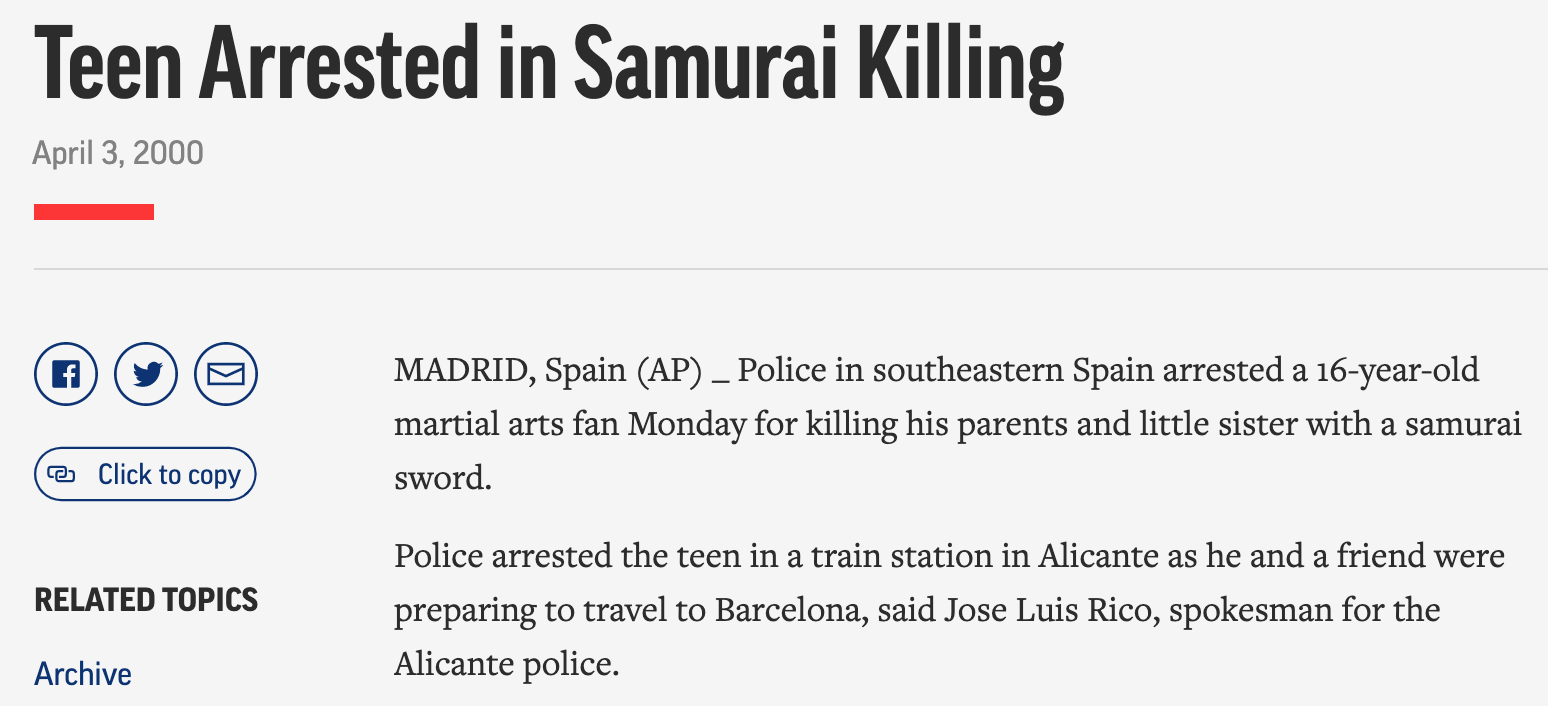
\includegraphics[width = \textwidth]{../img/katana}

\end{frame}
% ----------------------------------------------------

% ----------------------------------------------------
\begin{frame}
\frametitle{Why bother about theory?}
\centering

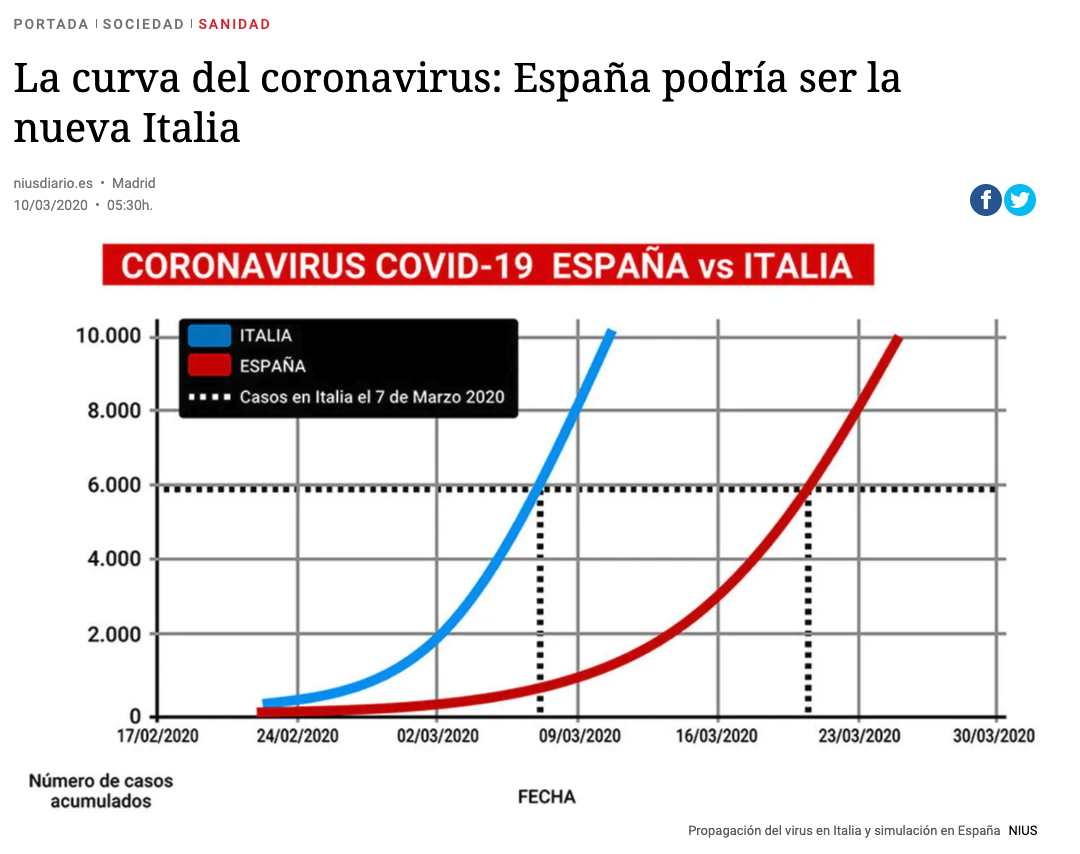
\includegraphics[width = 0.9\textwidth]{../img/covid_exp}

\end{frame}
% ----------------------------------------------------

% ----------------------------------------------------
\begin{frame}
\frametitle{Computational methods and theory}
\centering

\begin{itemize}
  \item Limitations of \textit{data mining}
  \item Focus on the what rather that on the why
  \item Problems with machine learning
  \begin{itemize}
    \item Example of predicting ice cream sales
  \end{itemize}
\end{itemize}

\end{frame}
% ----------------------------------------------------

% ----------------------------------------------------
\begin{frame}
\frametitle{Why bother about theory?}
\centering

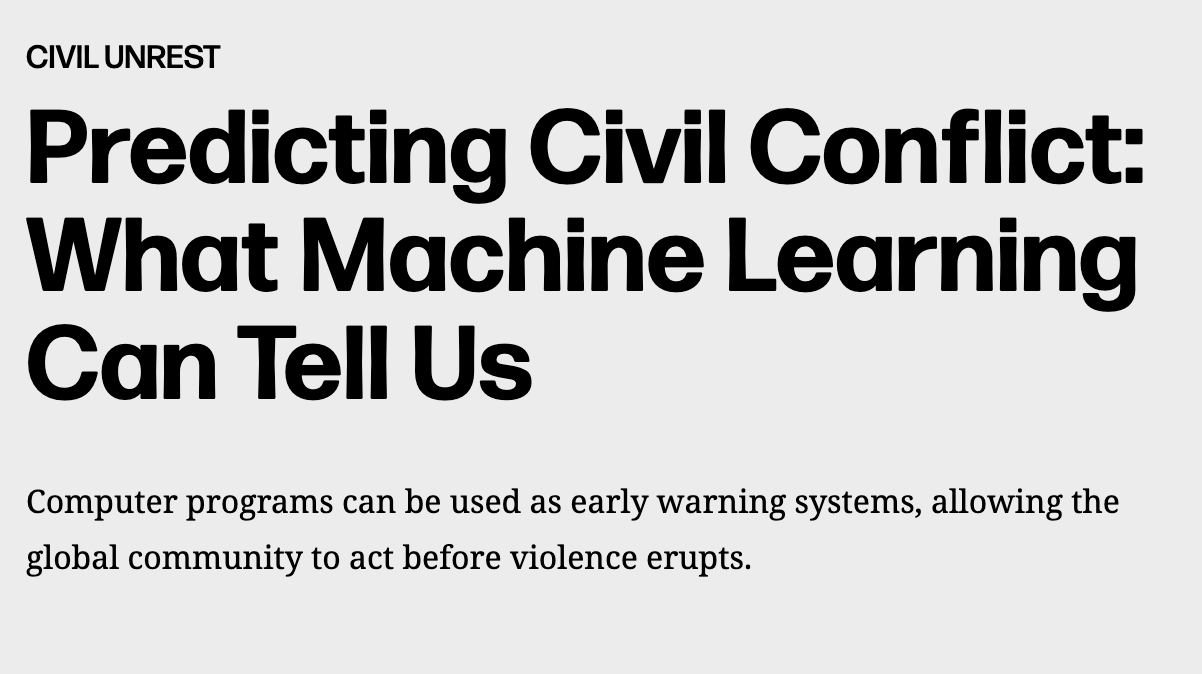
\includegraphics[width = \textwidth]{../img/predicting_conflict}

\end{frame}
% ----------------------------------------------------

% ----------------------------------------------------
\begin{frame}
\frametitle{Mechanisms briefly}
\centering

\begin{itemize}
  \item A \textbf{mechanism} is basically the \textbf{how} (or why) of a relationship
  \item e.g., we know that the flu gives us fever
  \begin{itemize}
    \item flu $>$ fever
  \end{itemize}
  \item<2-> What's the mechanism?
  \begin{itemize}
    \item flu $>$ \textit{immune system detects infection} $>$ $\Delta$ \textit{body temp} $>$ fever
  \end{itemize}
  \item<3-> Good thing about mechanisms is that we can try to test them
\end{itemize}

\end{frame}
% ----------------------------------------------------

% ----------------------------------------------------
\begin{frame}
\frametitle{Testing mechanisms ($\approx$ sub-research questions)}
\centering

\begin{itemize}
  \item Let's go back to the Erasmus example
  \item If our theory is that the effect of going on Eramus is higher for high-income students due to their access to social networks,
  \item[] \textbf{what's the mechanism?}
  \item And how could we try to \textbf{test it}?
  \begin{itemize}
    \item (Think about the sub-RQs)
  \end{itemize}
\end{itemize}

\end{frame}
% ----------------------------------------------------

% ----------------------------------------------------
\begin{frame}
\frametitle{Recap}
\centering

\begin{itemize}
  \item Questions on theory, RQ, or mechanisms?
\end{itemize}

\end{frame}
% ----------------------------------------------------

\section{Concepts and operationalization}

% ----------------------------------------------------
\begin{frame}
\frametitle{Concepts}
\centering

\begin{itemize}
  \item What are \textbf{concepts}?
  \item No need to get into epistemological discussions, but basically concepts are the \textbf{building blocks of analytical arguments}
  \item So part of the theoretical framework
  \item[]
  \item<2-> Some times they are a no brainer (income), but in many cases we have to think about them
  \begin{itemize}
    \item \textit{Household} income? What's considered a household?
    \item More problematic: Ideology? Democracy?
  \end{itemize}
  \item<3-> Also minor point: \textit{concept} $\neq$ \textit{term}
  \begin{itemize}
    \item Think about the labels we use to refer to some particular concept, e.g. authoritarian regime (i.e. dictatorship), rationality, etc
  \end{itemize}
\end{itemize}


\end{frame}
% ----------------------------------------------------

% ----------------------------------------------------
\begin{frame}
\frametitle{Concepts types}
\centering

\begin{itemize}
  \item No fixed categories, but some people talk of:
  \item[1.] \textbf{Rule-based} (definition)
  \begin{itemize}
    \item e.g. what are the rules we could use to define a household?
  \end{itemize}
  \item[2.] \textbf{Ideal types} (or family resemblance?)
  \begin{itemize}
    \item How do household look like? Can we intuitively identify them?
  \end{itemize}
  \item Rather that two exclusive types of concepts, they are two ways to think about them which are usually useful in improving concepts
\end{itemize}

\end{frame}
% ----------------------------------------------------

% ----------------------------------------------------
\begin{frame}
\frametitle{Operationalization}
\centering

\begin{itemize}
  \item To translate abstract concepts into concrete stuff we can observe and potentially measure
  \item Operationalize $\neq$ measure
  \begin{itemize}
    \item The fact that you can think of a concept in concrete terms does not mean you can always measure it easily
    \item Remember the algorithm that models rate of re-offenders
    \item Ideology of Twitter users? easy to op, hard to measure \textbf{(*)}
  \end{itemize}
  \item<2-> More like thinking of real-world attributes that map the conceptual dimensions we think about
  \begin{itemize}
    \item \textit{concept}: war intensity; \textit{operationalization}: number of battle deaths
  \end{itemize}
  \item<2-> the \textbf{Botswana example} on defining/operationalizing democracies
\end{itemize}

\end{frame}
% ----------------------------------------------------

% ----------------------------------------------------
\begin{frame}
\frametitle{Importance}
\centering

\begin{itemize}
  \item Might seem like something too abstract to care about (especially for computational social science), but it is actually not
  \item A \textbf{huge} part of good quantiative work relies on improving current concepts and their operationalization (which often leads to new ways of measuring them)
  \item Classic examples with theoretical importance (e.g. Putnam's \textit{social capital}), but also today's paper (`Roads to rule') is a good example of this
\end{itemize}

\end{frame}
% ----------------------------------------------------

% ----------------------------------------------------
\begin{frame}
\frametitle{Example}
\centering

\begin{itemize}
  \item Say we have a question about some $x$ cause of civil war outbreak
  \item That's two concepts we are actually talking about:
  \item[1.] \textbf{Civil war}
  \item[2.] \textbf{Outbreak}
  \item How could we define them? And operationalize them?
\end{itemize}

\end{frame}
% ----------------------------------------------------

% ----------------------------------------------------
\begin{frame}
\frametitle{Another example of a contentious concept}
\centering

\begin{itemize}
  \item What is \textbf{populism}? How can we operationalize it?
  \begin{itemize}
    \item e.g. how could we code a list of \textit{populist} political parties? or leaders?
  \end{itemize}
  \item[]
  \item[] (re: moving concepts up and down different levels of analysis)
\end{itemize}

\end{frame}
% ----------------------------------------------------

\section{Measurement}

% ----------------------------------------------------
\begin{frame}
\frametitle{Measurement issues}
\centering

\begin{itemize}
  \item[1.] Measuring what you really want to measure
  \begin{itemize}
    \item Careful with the use of proxies
  \end{itemize}
  \item[2.] Keep in mind what units you're not observing
  \begin{itemize}
    \item Missing data, sampling bias
  \end{itemize}
  \item[3.] Choosing the right unit of analysis
  \begin{itemize}
    \item Depends on the theory
  \end{itemize}
\end{itemize}

\end{frame}
% ----------------------------------------------------

% ----------------------------------------------------
\begin{frame}
\frametitle{Measurement issue \#1}
\centering

Measuring the \BGyellow{right stuff}

\end{frame}
% ----------------------------------------------------
  

% ----------------------------------------------------
\begin{frame}
\frametitle{Measuring the right stuff}
\centering

\begin{itemize}
  \item Not a lot to say here, other than to \textbf{pay attention}
  \item We normally look at one variable superficially without thinking about how it was created
  \item How was it exactly measured?
  \begin{itemize}
    \item Survey wordings
    \item Coding issues (e.g. level of democracy)
    \item Type of raw data used
  \end{itemize}
  \item And more importantly, are there \textbf{biases related to our question}?
\end{itemize}

\end{frame}
% ----------------------------------------------------

% ----------------------------------------------------
\begin{frame}
\frametitle{(A few strategies to measure stuff not directly observable)}
\centering

\begin{itemize}
  \item<2->[] \textit{Example}: we want to measure the ideological or policy positions of political parties
  \item<3-> \textbf{Expert surveys}
  \begin{itemize}
    \item You send questionnaires to experts who then reply, aggregate using average or similar
  \end{itemize}
  \item<4-> \textbf{Coding written texts}
  \begin{itemize}
    \item Manifesto project, but also others based on NLP
  \end{itemize}
  \item<5-> \textbf{Observing roll call voting}
  \begin{itemize}
    \item Voteview project
  \end{itemize}
  \item[]
  \item<5-> All these point to slightly different concepts or operationalizations
  \item<5-> We'll see a different strategy based on \textit{latent variables} in a moment
\end{itemize}

\end{frame}
% ----------------------------------------------------

% ----------------------------------------------------
\begin{frame}
\frametitle{Measuring the right stuff: Example}
\centering

\begin{itemize}
  \item You are doing research on whether discrimination of minorities has a negative effect on overall economic performance of a country
  \item<2-> You find a dataset that lists all minorities in a given country and gives them a yearly score of discrimination from 0 to 10
  \begin{itemize}
    \item In the codebook says that discrimination is conceptualized as `unequal access to state power, which ranges from actual, active discrimination (including mass violence perpetrated against members of the minority group) to lack of access to key political positions in the central government`
  \end{itemize}
  \item<3-> You also learn that the dataset was coded through \textbf{expert surveys}, sending a questionnaire to 2--3 researchers from each country
  \item<4-> \textbf{What do you think?}
\end{itemize}

\end{frame}
% ----------------------------------------------------

% ----------------------------------------------------
\begin{frame}
\frametitle{Measuring the right stuff: Example}
\centering

\begin{itemize}
  \item Now imagine you use the same dataset to analyze whether more extreme forms of discrimination make violence against minorities more likely
  \begin{itemize}
    \item You take the violence data from another dataset that e.g. codes actual violence events from newspapers
  \end{itemize}
  \item You find a \textit{positive relationship} in the results
  \item Thoughts?
  \item<2-> (Go back to previous definition)
  \item<3-> Another issue: difference depending on whether you do \textit{within vs between comparisons}
\end{itemize}

\end{frame}
% ----------------------------------------------------

% ----------------------------------------------------
\begin{frame}
\frametitle{Measuring the right stuff: Another example}
\centering

\begin{itemize}
  \item Recent debate on \textbf{democratic backsliding}
  \item Problem: how do we measure democracy?
  \item Available data: many international datasets on democracy rely on subjetive \textbf{expert judgement}
\end{itemize}

\end{frame}
% ----------------------------------------------------

% ----------------------------------------------------
\imageframe{../img/little_meng}
% ----------------------------------------------------

% ----------------------------------------------------
\imageframe{../img/economist_backsliding}
% ----------------------------------------------------

% ----------------------------------------------------
\begin{frame}
\frametitle{EPR example? (https://icr.ethz.ch/data/epr/)}
\centering

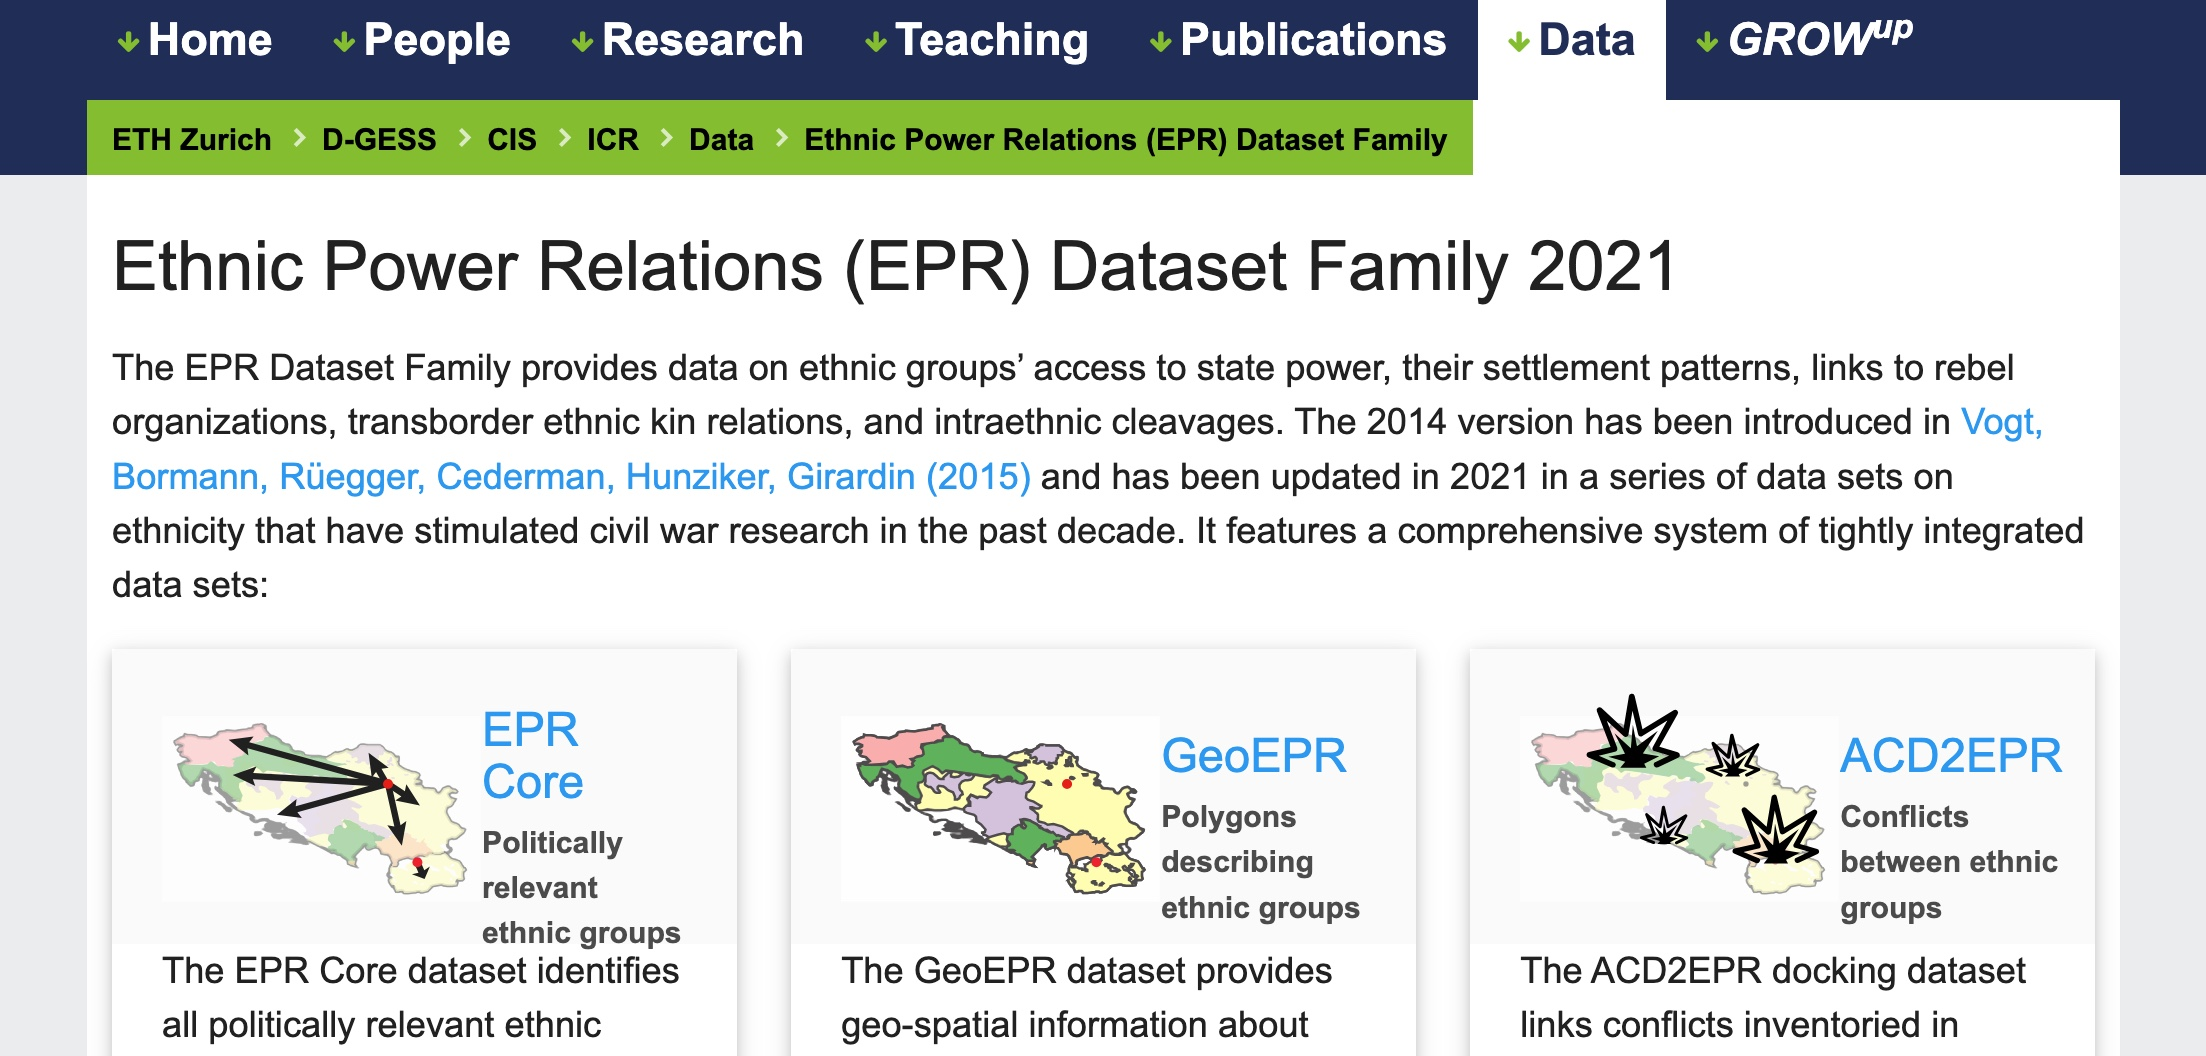
\includegraphics[width = \textwidth]{../img/epr1}

\end{frame}
% ----------------------------------------------------

% ----------------------------------------------------
\begin{frame}
\frametitle{EPR definitions}
\centering

{\small
\begin{itemize}
  \item \textbf{We define ethnicity} as a subjectively experienced sense of commonality based on a belief in common ancestry and shared culture. Different markers may be used to indicate such shared ancestry and culture: common language, similar phenotypical features, adherence to the same faith, and so on. \textbf{Our definition of ethnicity thus includes ethnolinguistic, ethnoreligious, and ethnosomatic (or “racial”) groups}, but not tribes and clans that conceive of ancestry in genealogical terms, nor regions that do not define commonality on the basis of shared ancestry.

  \item \textbf{An ethnic group is politically relevant if} either at least one significant political actor claims to represent the interests of that group in the national political arena or if group members are systematically and intentionally discriminated against in the domain of public politics.
\end{itemize}
}

\end{frame}
% ----------------------------------------------------

% ----------------------------------------------------
\begin{frame}
\frametitle{EPR definitions}
\centering

{\scriptsize
\begin{itemize}
\setlength\itemsep{0pt}
  \item \textbf{Monopoly}: Elite members hold monopoly power in the executive to the exclusion of members of all other ethnic groups.
  \item \textbf{Dominance}: ... dominant power in the executive but ... some limited inclusion of “token” members of other groups
  \item \textbf{Senior Partner}: Representatives of the group participate as senior partners in a formal or informal power-sharing arrangement ...(any arrangement that divides executive power among leaders who claim to represent particular ethnic groups and who have real influence on political decision making)
  \item \textbf{Junior Partner}: ... as junior partners in government.
  \item \textbf{Powerless}: Elite representatives hold no political power (or do not have influence on decision making) at the national level of executive power - although without being explicitly discriminated against.
  \item \textbf{Discrimination}: Group members are subjected to active, intentional, and targeted discrimination (formal or informal) by the state, with the intent of excluding them from political power (but not from socio-economic sphere).
  \item \textbf{Self-exclusion}: groups that have excluded themselves from central state power, in the sense that they control a particular territory of the state which they have declared independent
\end{itemize}
}

\end{frame}
% ----------------------------------------------------

% ----------------------------------------------------
\begin{frame}
\frametitle{EPR in Spain?}
\centering

\begin{itemize}
  \item How would you code Spain? (Or your own country, in case it's multi-ethnic)
  \item Two main things?
  \item[1.] How many \textit{politically relevant} ethnic groups?
  \item[2.] Political status by period?
\end{itemize}

\end{frame}
% ----------------------------------------------------

% ----------------------------------------------------
\imageframe{../img/epr2}
% ----------------------------------------------------

% ----------------------------------------------------
\begin{frame}
\frametitle{Democratic backsliding}
\centering

\begin{itemize}
  \item `Objective' and `subjective' operationalization \& measurement
  \item `Objective' measures usually rely on a \textit{minimalist} conceptualization of democracy
  \begin{itemize}
    \item e.g. celebration of contested elections
  \end{itemize}
  \item `Subjective' measures tap into \textit{maximalist} definitions of democracy that incorporate more dimensions
  \begin{itemize}
    \item regular, contested elections; but also rule of law, participation, media, etc
  \end{itemize}
  \item Problem: Autocrats are usually pretty creative
\end{itemize}

\end{frame}
% ----------------------------------------------------

% ----------------------------------------------------
\begin{frame}
\frametitle{The case for objective measures}
\centering

\begin{itemize}
  \item One example from the ACLP (Alvarez, Cheibub, Limongi, Przeworski) Democracy and Dictatorship Dataset
  \item Coding democracy based on four objective, observable rules:
  \item[1.] {\small The chief executive must be chosen by popular election or by a body that was itself popularly elected.}
  \item[2.] {\small The legislature must be popularly elected.}
  \item[3.] {\small There must be more than one party competing in the elections.}
  \item[4.] {\small An alternation in power under electoral rules identical to the ones that brought the incumbent to office must have taken place.}
\end{itemize}

\end{frame}
% ----------------------------------------------------

% ----------------------------------------------------
\imageframe{../img/democratic_backsliding}
% ----------------------------------------------------

% ----------------------------------------------------
\begin{frame}
\frametitle{One view on this (by V-Dem people)}
\centering

\begin{itemize}
  \item Even if using expert surveys, you can take some measures
  \begin{itemize}
    \item Aim for \textit{replicability}
    \item Incorporate measures of uncertainty
    \item Build it differently: e.g. incorporate different dimensions, use an ordinal scale, aggregate differently, etc
  \end{itemize}
  \item `Objective measures' are not that objective
  \begin{itemize}
    \item Botswana example, and systematic downward bias against young democracies with economic growth
    \item e.g. how do you detect fraud? election forensics methods (based on distribution) can be incorporated by autocrats in later elections
  \end{itemize}
  \item[]
  \item {\small To know more: Knutsen \textit{et al.} `Conceptual and Measurement Issues in Assessing Democratic Backsliding.' V-Dem Working Paper, May 2023.}
  \begin{itemize}
    \item \url{v-dem.net/media/publications/wp_140.pdf}
  \end{itemize}
\end{itemize}

\end{frame}
% ----------------------------------------------------

% ----------------------------------------------------
\begin{frame}
\frametitle{Proxies}
\centering

\begin{itemize}
  \item A \textbf{proxy variable} is a variable that we use to substitute another variable we cannot observe or measure
  \item This is a matter of creativity, but the important thing is to think about \textbf{potential biases}
  \item A real example:
  \begin{itemize}
    \item Trying to know if leftist/Basque nationalist priests during Francoist Spain had an effect on later terrorism
    \item First problem (among many): how do you measure the ideology of these people?
    \item Using the 1963 letter to the Vatican
  \end{itemize}
\end{itemize}

\end{frame}
% ----------------------------------------------------

% ----------------------------------------------------
\begin{frame}
\frametitle{Latent variables}
\centering

\begin{itemize}
  \item Some concepts are just not directly observable
  \begin{itemize}
    \item (or very expensive / unfeasible to do so)
  \end{itemize}
  \item Another option is to create the variable out of other observables
  \item This is sometimes called \textbf{latent variables}
\end{itemize}

\end{frame}
% ----------------------------------------------------

% ----------------------------------------------------
\begin{frame}
\frametitle{Latent variables}
\centering

\begin{itemize}
  \item Let's look at one example: imagine you want to do research on whether left-wing or right-wing people tweet differently (or some other outcome, e.g. echo chambers idea)
  \item It's easy to get data on the outcome variable (Tweet content, frequency, ...)
  \begin{itemize}
    \item if you don't know how now, you'll learn in the spring
  \end{itemize}
  \item But \textbf{how do you code ideology?}
  \begin{itemize}
    \item<2-> Some people have done it focusing only on a subset, e.g. politicians, for which you have information (problem of selection)
    \item<3-> Of even some others have linked survey data to Twitter activity, asking for consent (problem of cost, non-response)
  \end{itemize}
\end{itemize}

\end{frame}
% ----------------------------------------------------

% ----------------------------------------------------
\imageframe{../img/barbera_tw1}
% ----------------------------------------------------

% ----------------------------------------------------
\imageframe{../img/barbera_tw2}
% ----------------------------------------------------

% ----------------------------------------------------
\begin{frame}
\frametitle{Validating measure}
\centering

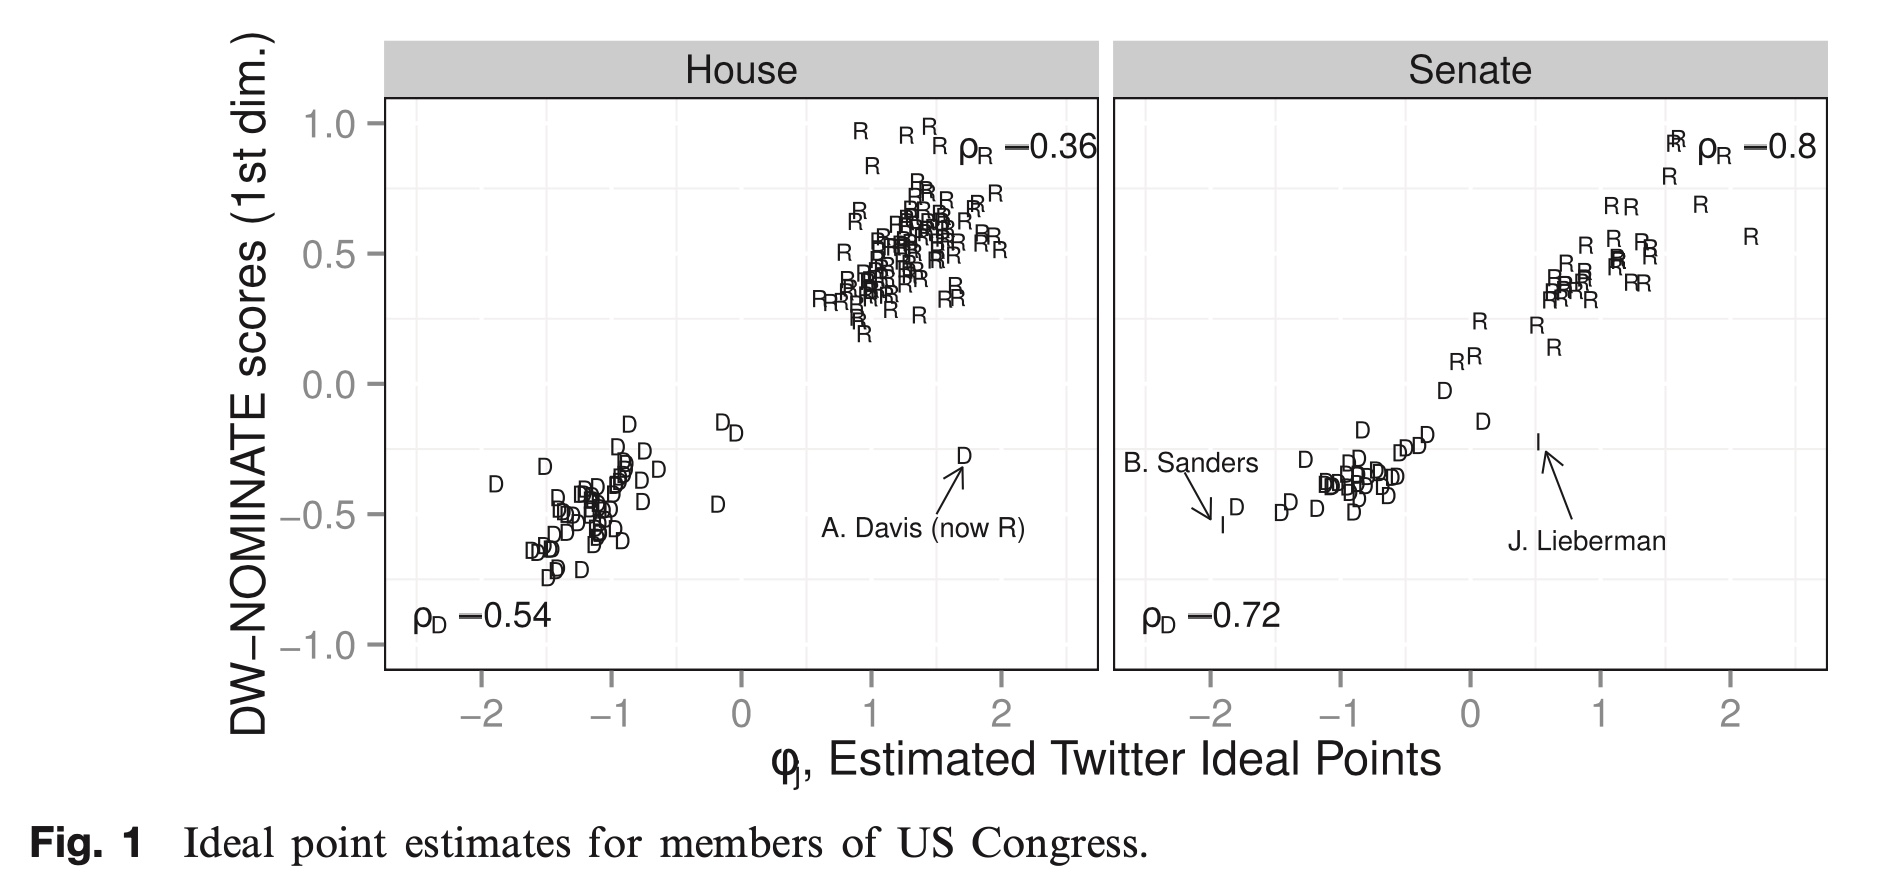
\includegraphics[width = \textwidth]{../img/barbera_tw3}

\end{frame}
% ----------------------------------------------------

% ----------------------------------------------------
\imageframe{../img/barbera_tw4}
% ----------------------------------------------------

% ----------------------------------------------------
\imageframe{../img/barbera_etal1}
% ----------------------------------------------------

% ----------------------------------------------------
\imageframe{../img/barbera_etal2}
% ----------------------------------------------------

% ----------------------------------------------------
\begin{frame}
\frametitle{Measurement issue \#2}
\centering

What units are you \BGyellow{not} measuring?

\end{frame}
% ----------------------------------------------------

% ----------------------------------------------------
\begin{frame}
\frametitle{Beyond our observations: missing data}
\centering

\begin{itemize}
  \item \textbf{Missing data} is when we don't have data for some observations
  \begin{itemize}
    \item often more important that it looks, important to understand if it's biasing our analyses
  \end{itemize}
  \item[] Three types:
  \item<2->[1.] Missing \textbf{completely at random}
  \begin{itemize}
    \item No problem, random observations are missing
    \item[] (Probably not very often)
  \end{itemize}
  \item<3->[2.] Missing \textbf{at random}
  \begin{itemize}
    \item One variable explains whether obs are missing or not, but it's not related to our question
  \end{itemize}
  \item<4->[3.] Missing \textbf{not at random}
  \begin{itemize}
    \item The variable that explains `missingness' is key to our question
  \end{itemize}
  \item[]
  \item<4-> {\small Example: smoking status missing, gender (MAR), emergency (MNAR)}
\end{itemize}

% {\color{red}{\textbf{EXAMPLES? WITH DAGS?}}}

\end{frame}
% ----------------------------------------------------

% ----------------------------------------------------
\begin{frame}
\frametitle{Beyond our observations: sampling bias}
\centering

\begin{itemize}
  \item \textbf{Sampling bias} could be thought of as missing data or, rather, as a controlling variable we'll indirectly including
  \item Easy case: we're dealing with a pre-designed sample that might have some biases
  \begin{itemize}
    \item Online survey and +65
  \end{itemize}
  \item<2-> More easy to miss: there is an `invisible variable' determining which observations we have or not
  \begin{itemize}
    \item e.g. when using Twitter data,
  \end{itemize}
  \item<2-> We'll talk more about how this affects inference
  \begin{itemize}
    \item Collider bias example?
  \end{itemize}
\end{itemize}

\end{frame}
% ----------------------------------------------------

% ----------------------------------------------------
\begin{frame}
\frametitle{Measurement issue \#3}
\centering

At \BGyellow{which level} should we measure?

\end{frame}
% ----------------------------------------------------

% ----------------------------------------------------
\begin{frame}
\frametitle{Unit of analyses}
\centering

\begin{itemize}
  \item Level at which we have our observations
  \item Deeply related to the variables we have
  \begin{itemize}
    \item Even though not all variables have to/can be measured at the same level
    \item<2-> e.g. individual-level data and household income
  \end{itemize}
  \item<3-> Most important thing: we need to \textbf{choose the right unit of analyses} depending on the theory (and mechanism) we are testing
  \begin{itemize}
    \item Getting the variation that matters (example of online bookings?)
  \end{itemize}
\end{itemize}


\end{frame}
% ----------------------------------------------------

% ----------------------------------------------------
\begin{frame}
\frametitle{A more difficult example}
\centering

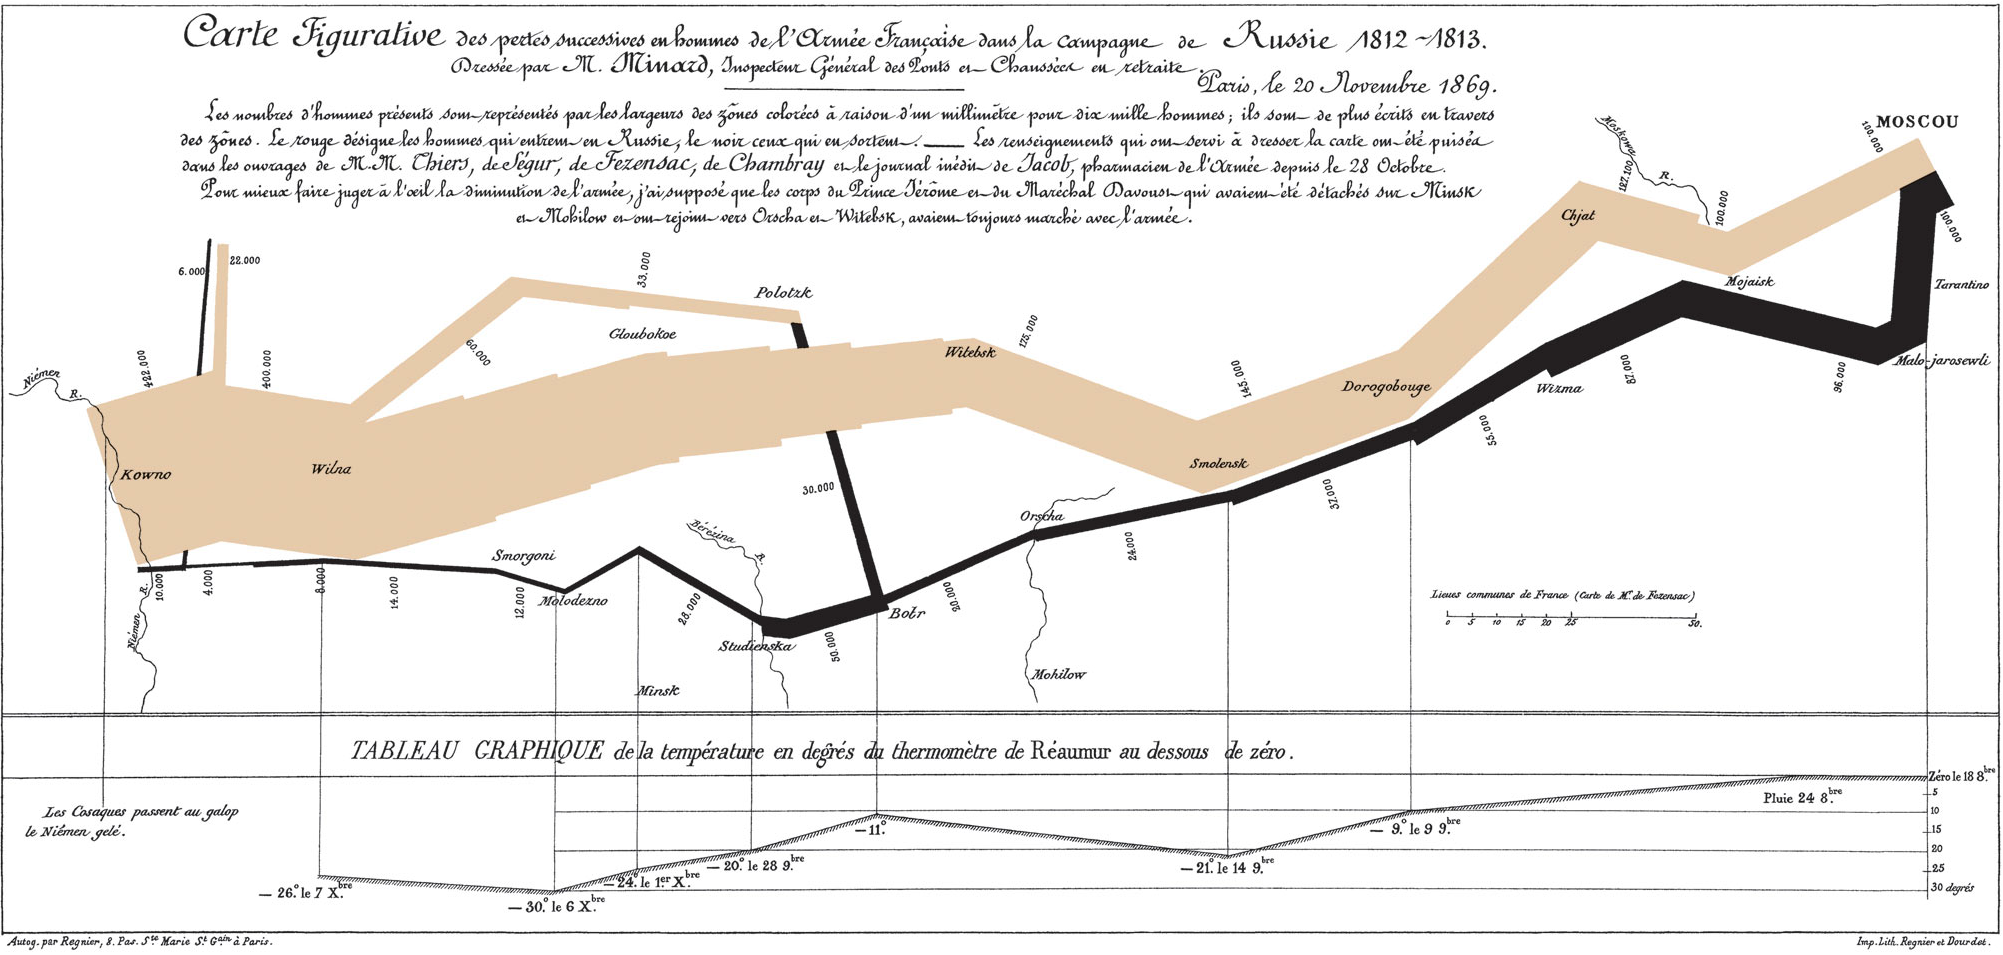
\includegraphics[width = \textwidth]{../img/Minard}

\vspace{10pt}

\begin{itemize}\footnotesize
  \item How many variables and what's the unit of observation?
  \begin{itemize}
    \item[Extra:] What's the causal argument being told here?
    \item[] Could we test it with the data we have?
  \end{itemize}
\end{itemize}

\end{frame}
% ----------------------------------------------------

% ----------------------------------------------------
\begin{frame}
\frametitle{Theories, hypotheses, and measurement}
\centering

\begin{itemize}
  \item Let's say I want to explain the effect of school choice on future salaries
  \item My argument is: going to private schools leads to higher salaries in the future because increased resources lead to better educational attainment through lower teacher/pupil ratio, which signals individuals as more skillful in the labour market, explaining higher salaries
  \item[]
  \item<2-> Hypotheses?
  \item<3-> Testing the relationship and the mechanism?
  \item[]<3-> And alternative explanations?
\end{itemize}

\end{frame}
% ----------------------------------------------------

% ----------------------------------------------------
\begin{frame}
\frametitle{Another example}
\centering

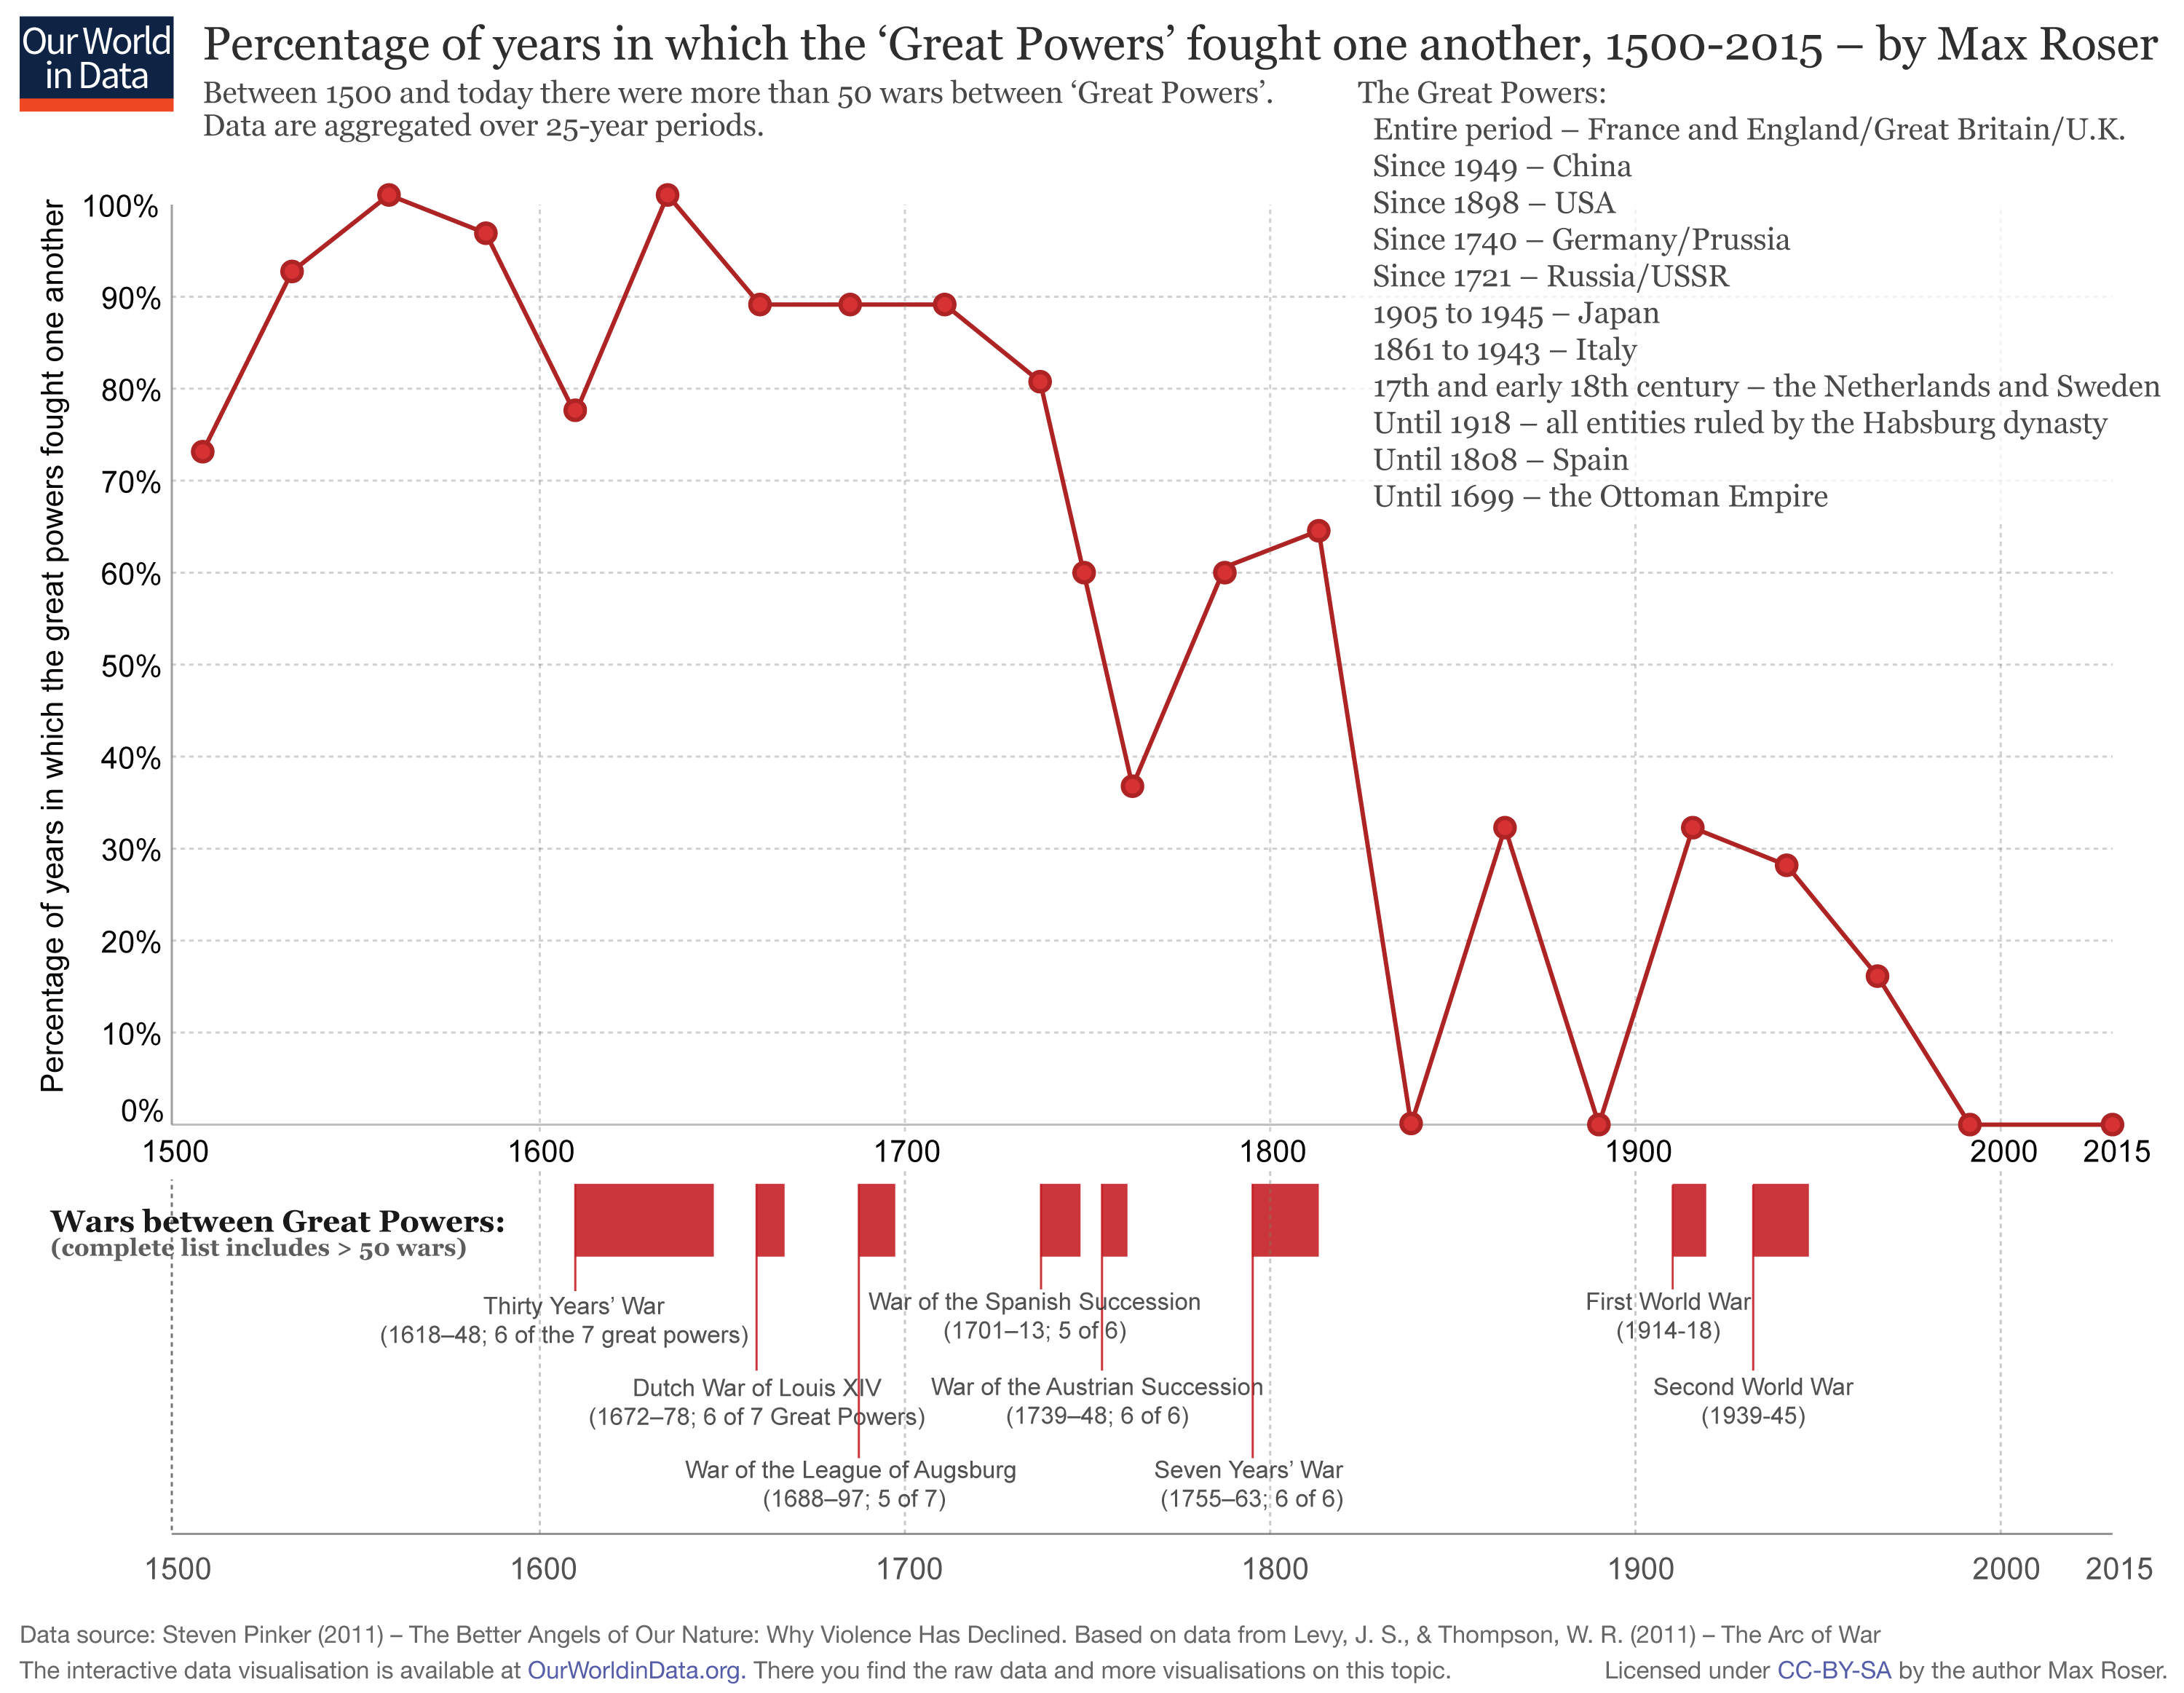
\includegraphics[width = \textwidth]{../img/declineofwar}

\end{frame}
% ----------------------------------------------------

% ----------------------------------------------------
\begin{frame}
\frametitle{Another example}
\centering

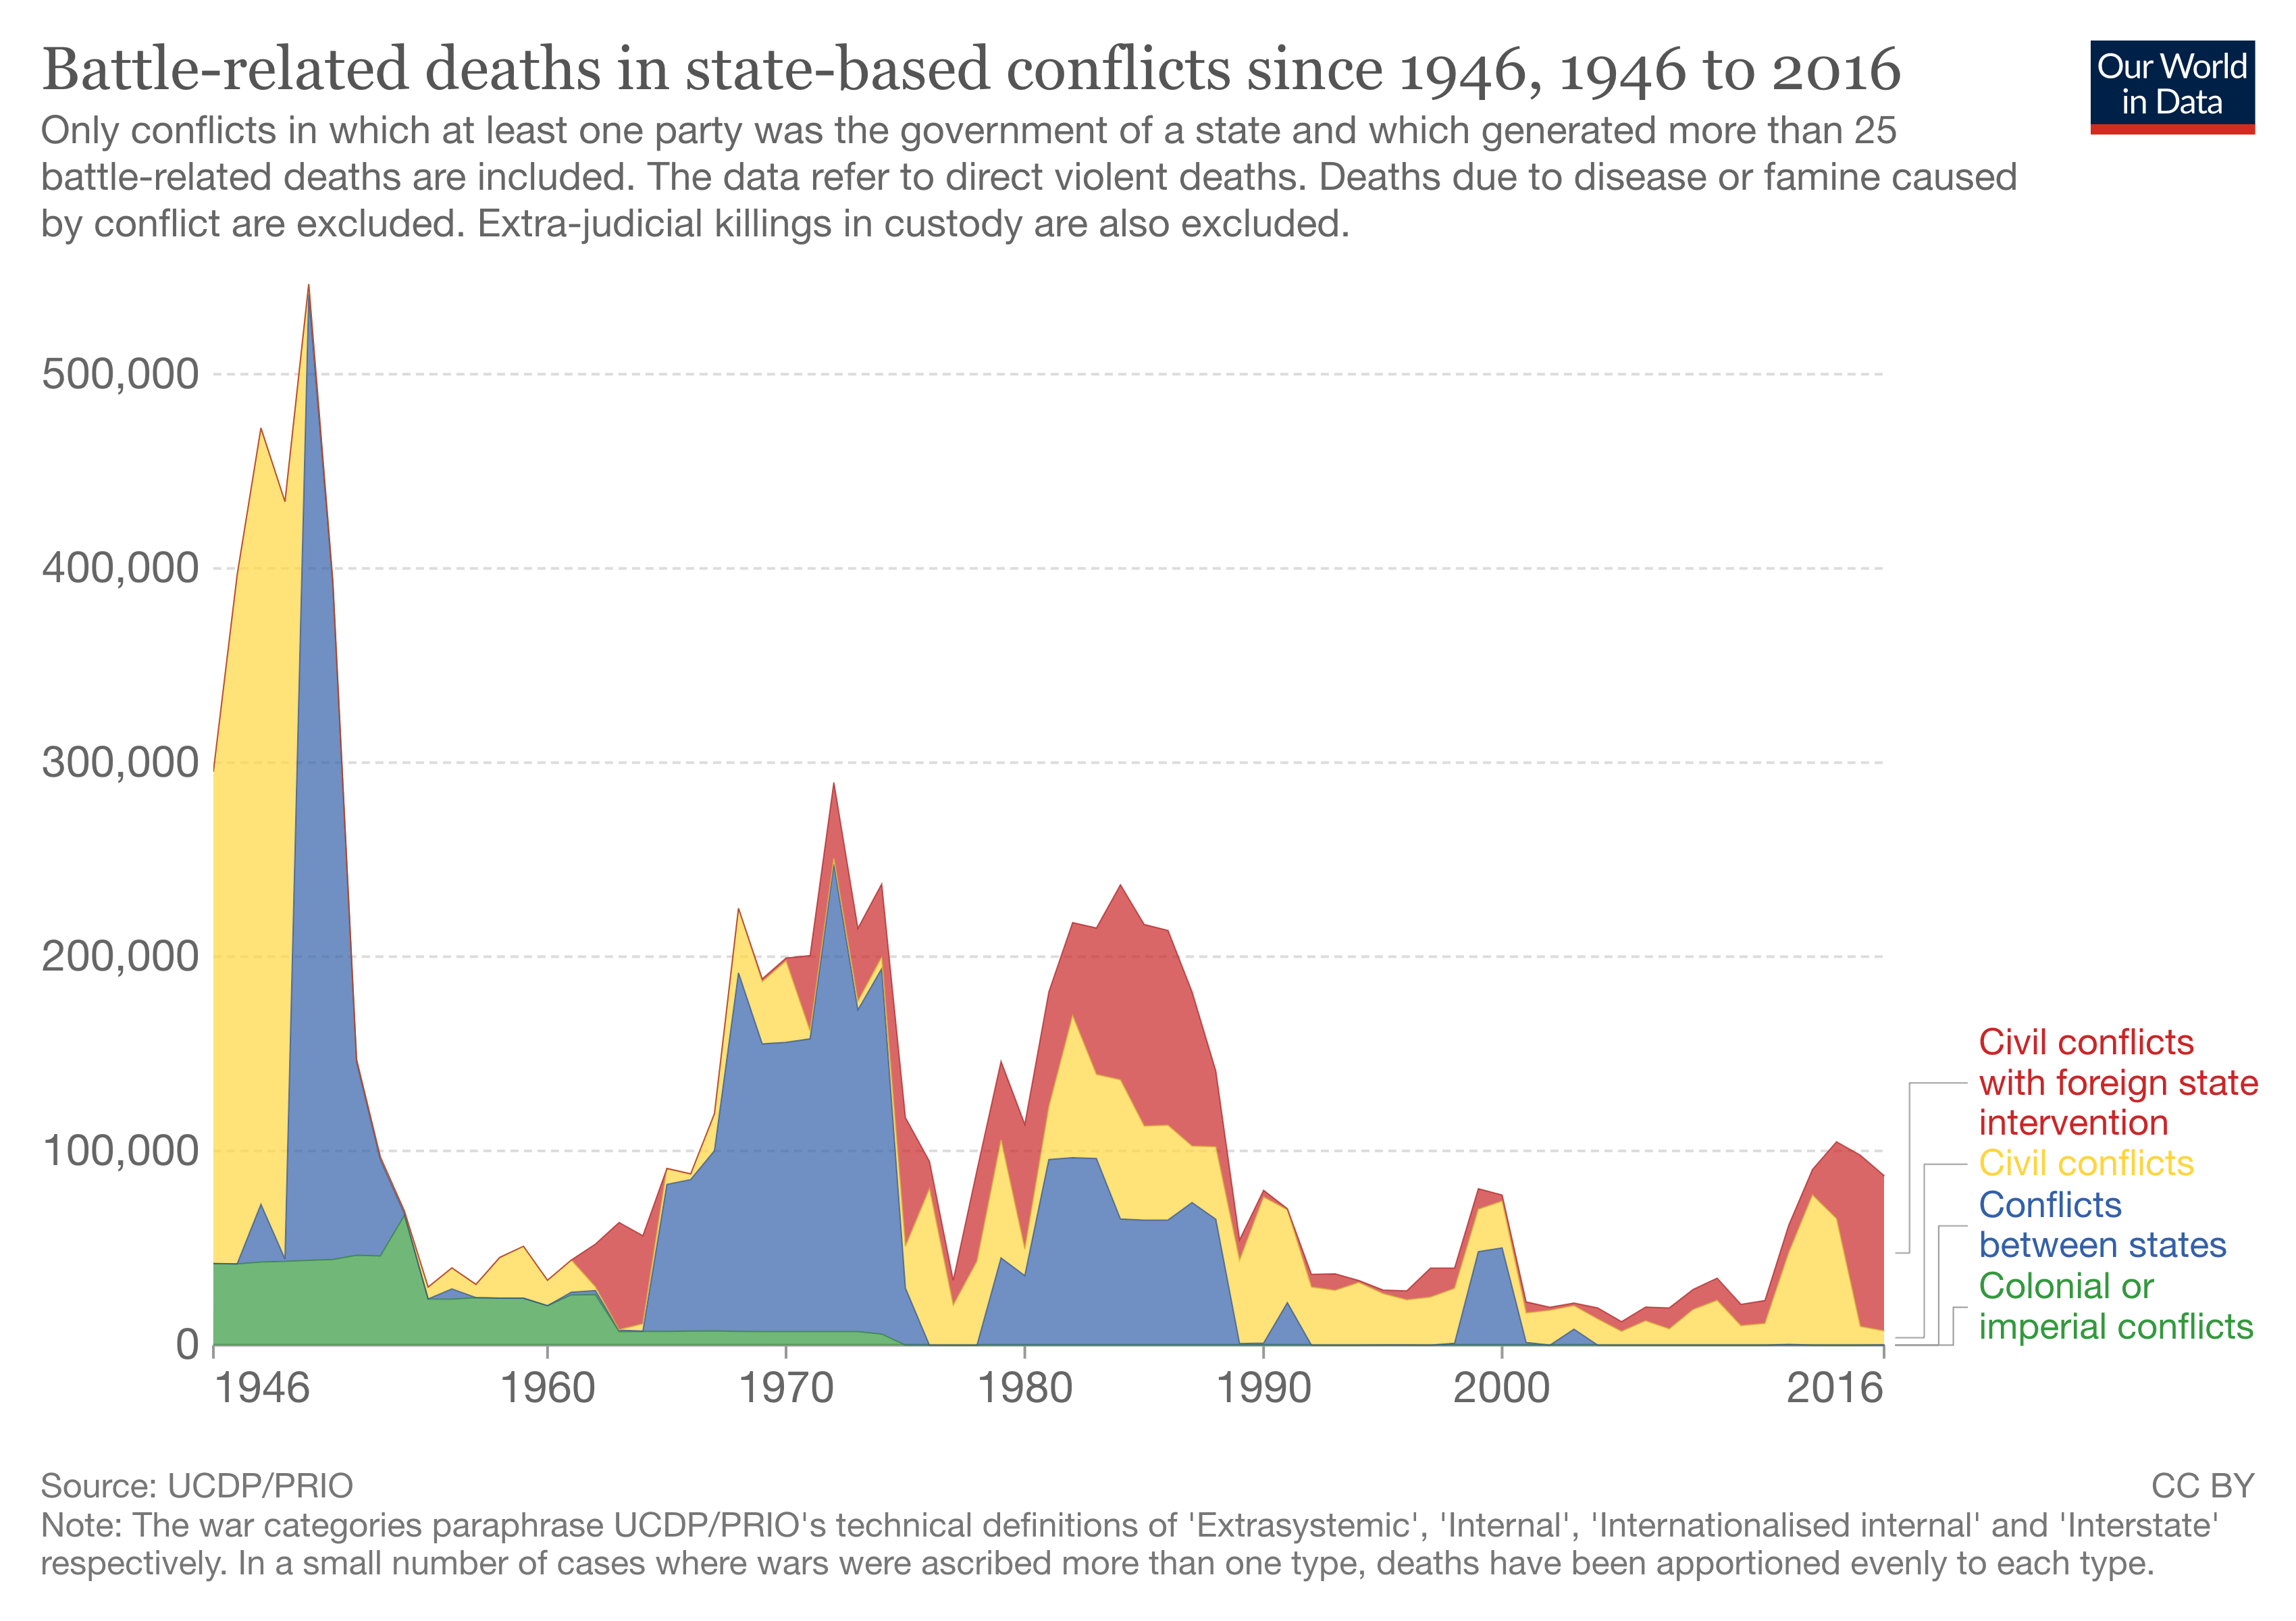
\includegraphics[width = \textwidth]{../img/battledeaths}

\end{frame}
% ----------------------------------------------------

% ----------------------------------------------------
\begin{frame}
\frametitle{Another example}
\centering

\begin{itemize}
  \item Now, let's say my theory is that inter-state war has declined because democratic countries are less likely to go to war because they face higher domestic costs for waging wars
  \item[]
  \item Hypotheses? Testing the mechanism? Unit of analyses? Measurement? Alternative explanations?
\end{itemize}

\end{frame}
% ----------------------------------------------------

% ----------------------------------------------------
\begin{frame}
\frametitle{Another example}
\centering

\begin{itemize}
  \item What if I say that it is because democracies do not fight \textit{each other}, as they have shared interests in the international system and shared conflict resolution mechanisms?
  \item[]
  \item And if I say that democratic countries face higher costs when fighting another democracy, but not otherwise?
  \item[]
  \item What should I observe in each case? At different levels? How to measure?
\end{itemize}

\end{frame}
% ----------------------------------------------------

% ----------------------------------------------------
\begin{frame}
\frametitle{Complexity of the social world and micro/macro}
\centering

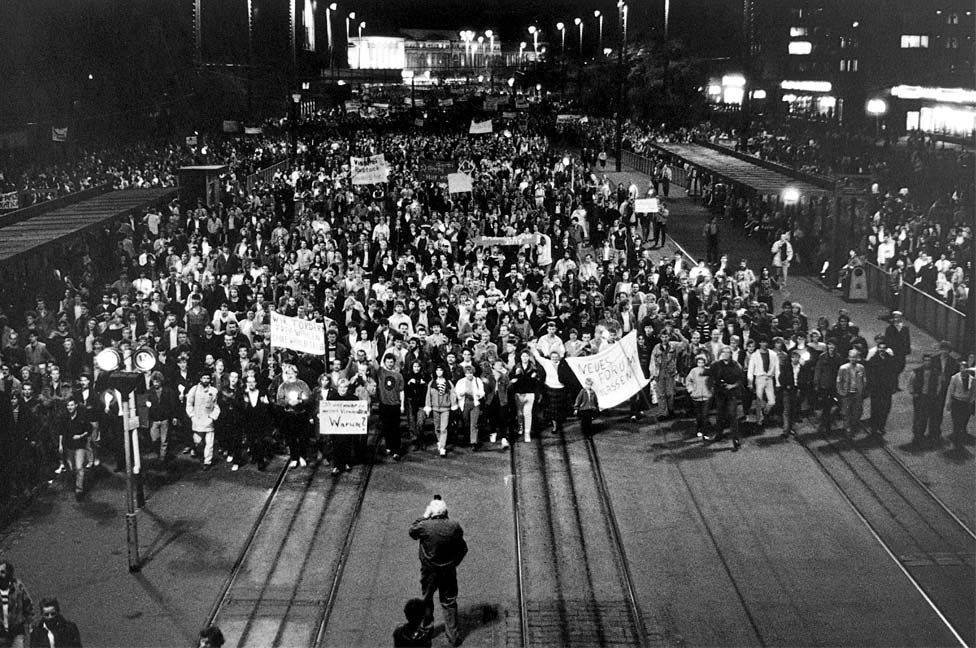
\includegraphics[width = 0.8\textwidth]{../img/leipzig1989}

\begin{itemize}
  \item Why do mass protests emerge?
\end{itemize}

\end{frame}
% ----------------------------------------------------

% ----------------------------------------------------
\begin{frame}
\frametitle{Levels of explanation}
\centering

\begin{itemize}
\item[] Can you think of...?
\item Macro-level mechanisms
\item Micro-level mechanisms
\item[]
\item<2-> What's the point of macro-level explanations, actually?
\end{itemize}

\end{frame}
% ----------------------------------------------------

% % ----------------------------------------------------
% \begin{frame}
% \frametitle{Extra: Measuring qualitative information}
% \centering
%
% \begin{itemize}
%   \item Imagine you have this question:
%   \item[] What are the differences between neoclassicism and romanticism in music?
%   \item[]
%   \item Could you try to make a quantitative question out of it?
% \end{itemize}
%
% \end{frame}
% % ----------------------------------------------------

\section{Description}

% ----------------------------------------------------
\begin{frame}
\frametitle{Describing variables}
\centering

\begin{itemize}
  \item What is a \textbf{variable}?
  \item Types?
  \begin{itemize}
    \item<2-> Continuous
    \item<3-> Count
    \item<4-> Ordinal
    \item<5-> Categorical (binary)
    \item<6-> Qualitative (* are really a variable?)
  \end{itemize}
  \item<7-> Why does it matter?
  \item<7-> Conceptual meaning vs statistical meaning
\end{itemize}

\end{frame}
% ----------------------------------------------------

% ----------------------------------------------------
\begin{frame}
\frametitle{Describing variables}
\centering

\begin{itemize}
  \item Main idea: you are describing the variable distribution (i.e. how the frequency of values looks like)
  \item You probably know this from basic statistics
  \begin{itemize}
    \item In practice, the measures of distribution do not matter so much
  \end{itemize}
  \item But one important thing: we are talking about \textbf{real-world observations}, so before you do anything (analyses, etc), do look at them
  \begin{itemize}
    \item At least, \textbf{plot the main variables}
    \item Is it coherent with the \textbf{theoretical} or \textbf{expected distribution}?
  \end{itemize}
\end{itemize}

\end{frame}
% ----------------------------------------------------

% ----------------------------------------------------
\begin{frame}
\frametitle{Describing variables}
\centering

\begin{itemize}
  \item Also, sometimes the distribution is important to think about actual effect sizes, so it's good to summarize variables {\footnotesize (mean, SD, IQR...)}
  \begin{itemize}
    \item Maybe this makes sense if you've learn logistic regression?
    \item We'll talk more tomorrow about the concept of average effect in causality
  \end{itemize}
  \item In a normal distribution, there's probably not much to say
  \item But what if a key independent variable has a bimodal distribution? What does this say about the \textbf{causal mechanism?}
  \begin{itemize}
    \item e.g. think about the effect of income on X in two societies: one is extremely unequal and the other is normally distributed
  \end{itemize}
\end{itemize}

\end{frame}
% ----------------------------------------------------

% ----------------------------------------------------
\begin{frame}
\frametitle{Describing relationships}
\centering

\begin{itemize}
  \item What is a \textbf{relationship}?
  \item Essentially that as you know about the values of one variable, you learn about the values of the other variables
  \item[] e.g. a \textit{negative} relationship means that you know that higher values in $x$ imply lower values in $y$
  \item[]
  \item[]<2-> Imagine you have a small car, and a friend of yours is coming and is bringing along his two kids. Concerned about space, you ask `\textit{how old are they?}` And the answer is: `\textit{They're 6 and 2}.`
  \begin{itemize}
    \item What do you imagine about size?
    \item<3-> Now imagine you ask `\textit{are they blonde, red-haired, or brown-haired?}'
  \end{itemize}
\end{itemize}

\end{frame}
% ----------------------------------------------------

% ----------------------------------------------------
\begin{frame}
\frametitle{Statistical relationship $\neq$ causal relationships}
\centering

\begin{itemize}
  \item<1-> Last example: Is there a causal relationship \textit{age} $\rightarrow$ \textit{size}?
  \item<2-> What if the variable you want to guess is \textbf{the time of the day}, and someone tells you that she just heard the rooster crow? Causal?
  \item[]
  \item<3-> Why are non-causal descriptive relationships \textbf{useful}?
\end{itemize}

\end{frame}
% ----------------------------------------------------

% % ----------------------------------------------------
% \begin{frame}
% \frametitle{Describing relationships}
% \centering
%
% conditional distributions
% conditional means
% conditional conditional means (controlling)
%
% \end{frame}
% % ----------------------------------------------------

% ----------------------------------------------------
\begin{frame}
\frametitle{Univariate description}
\centering

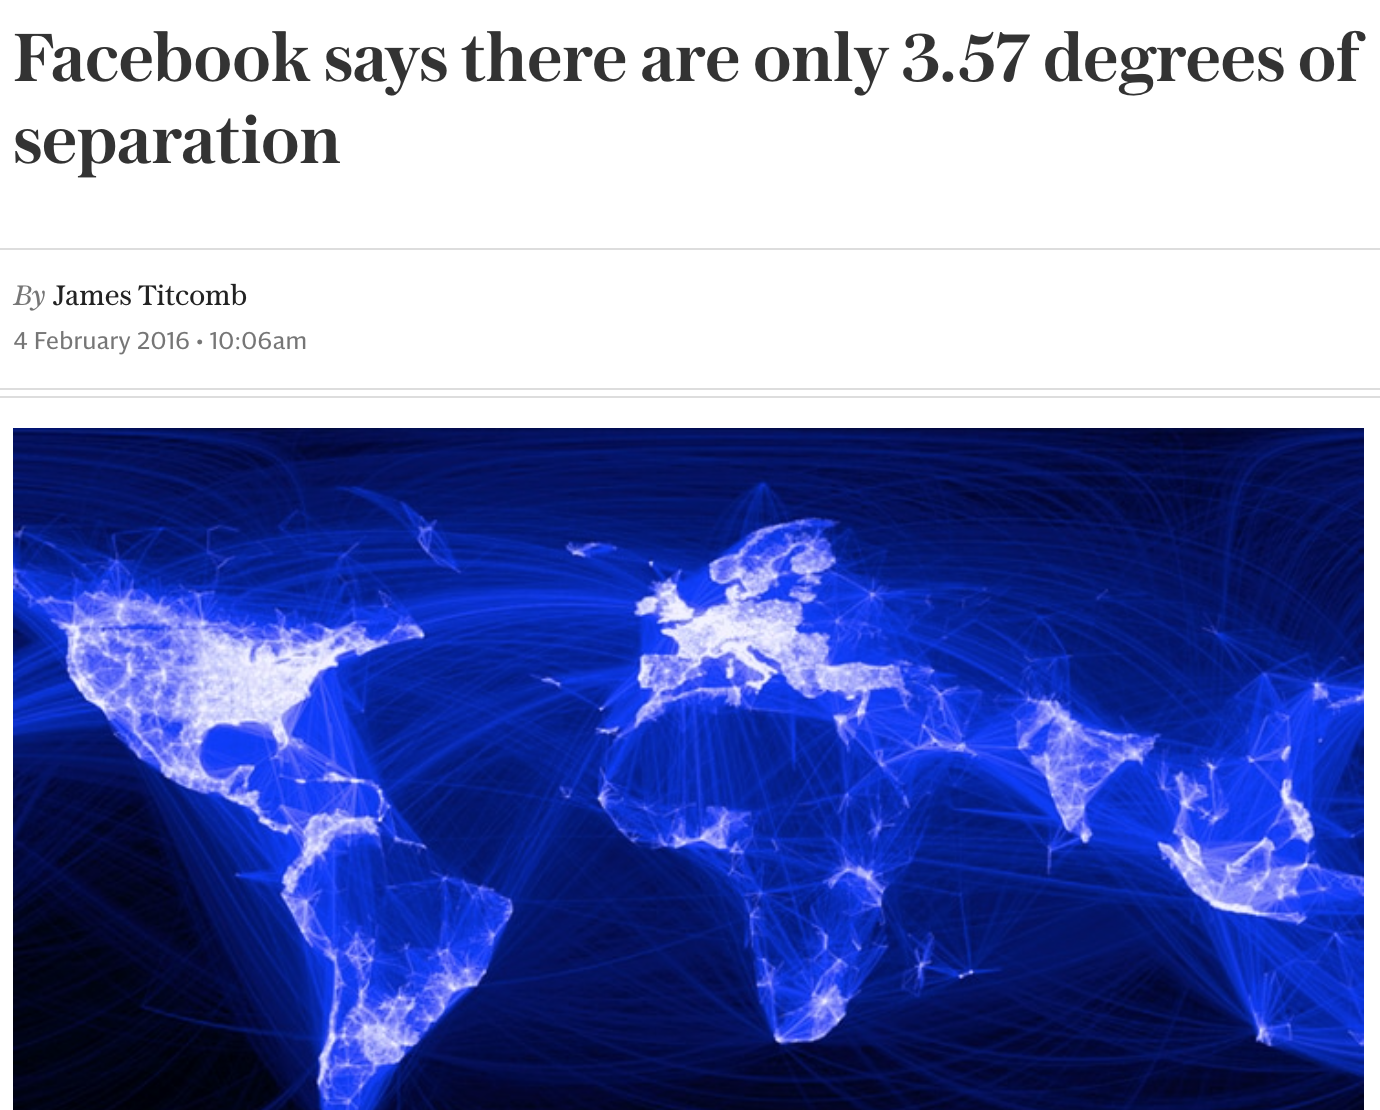
\includegraphics[width = \textwidth]{../img/sixdegrees}

\end{frame}
% ----------------------------------------------------

% ----------------------------------------------------
\begin{frame}
\frametitle{Univariate description}
\centering

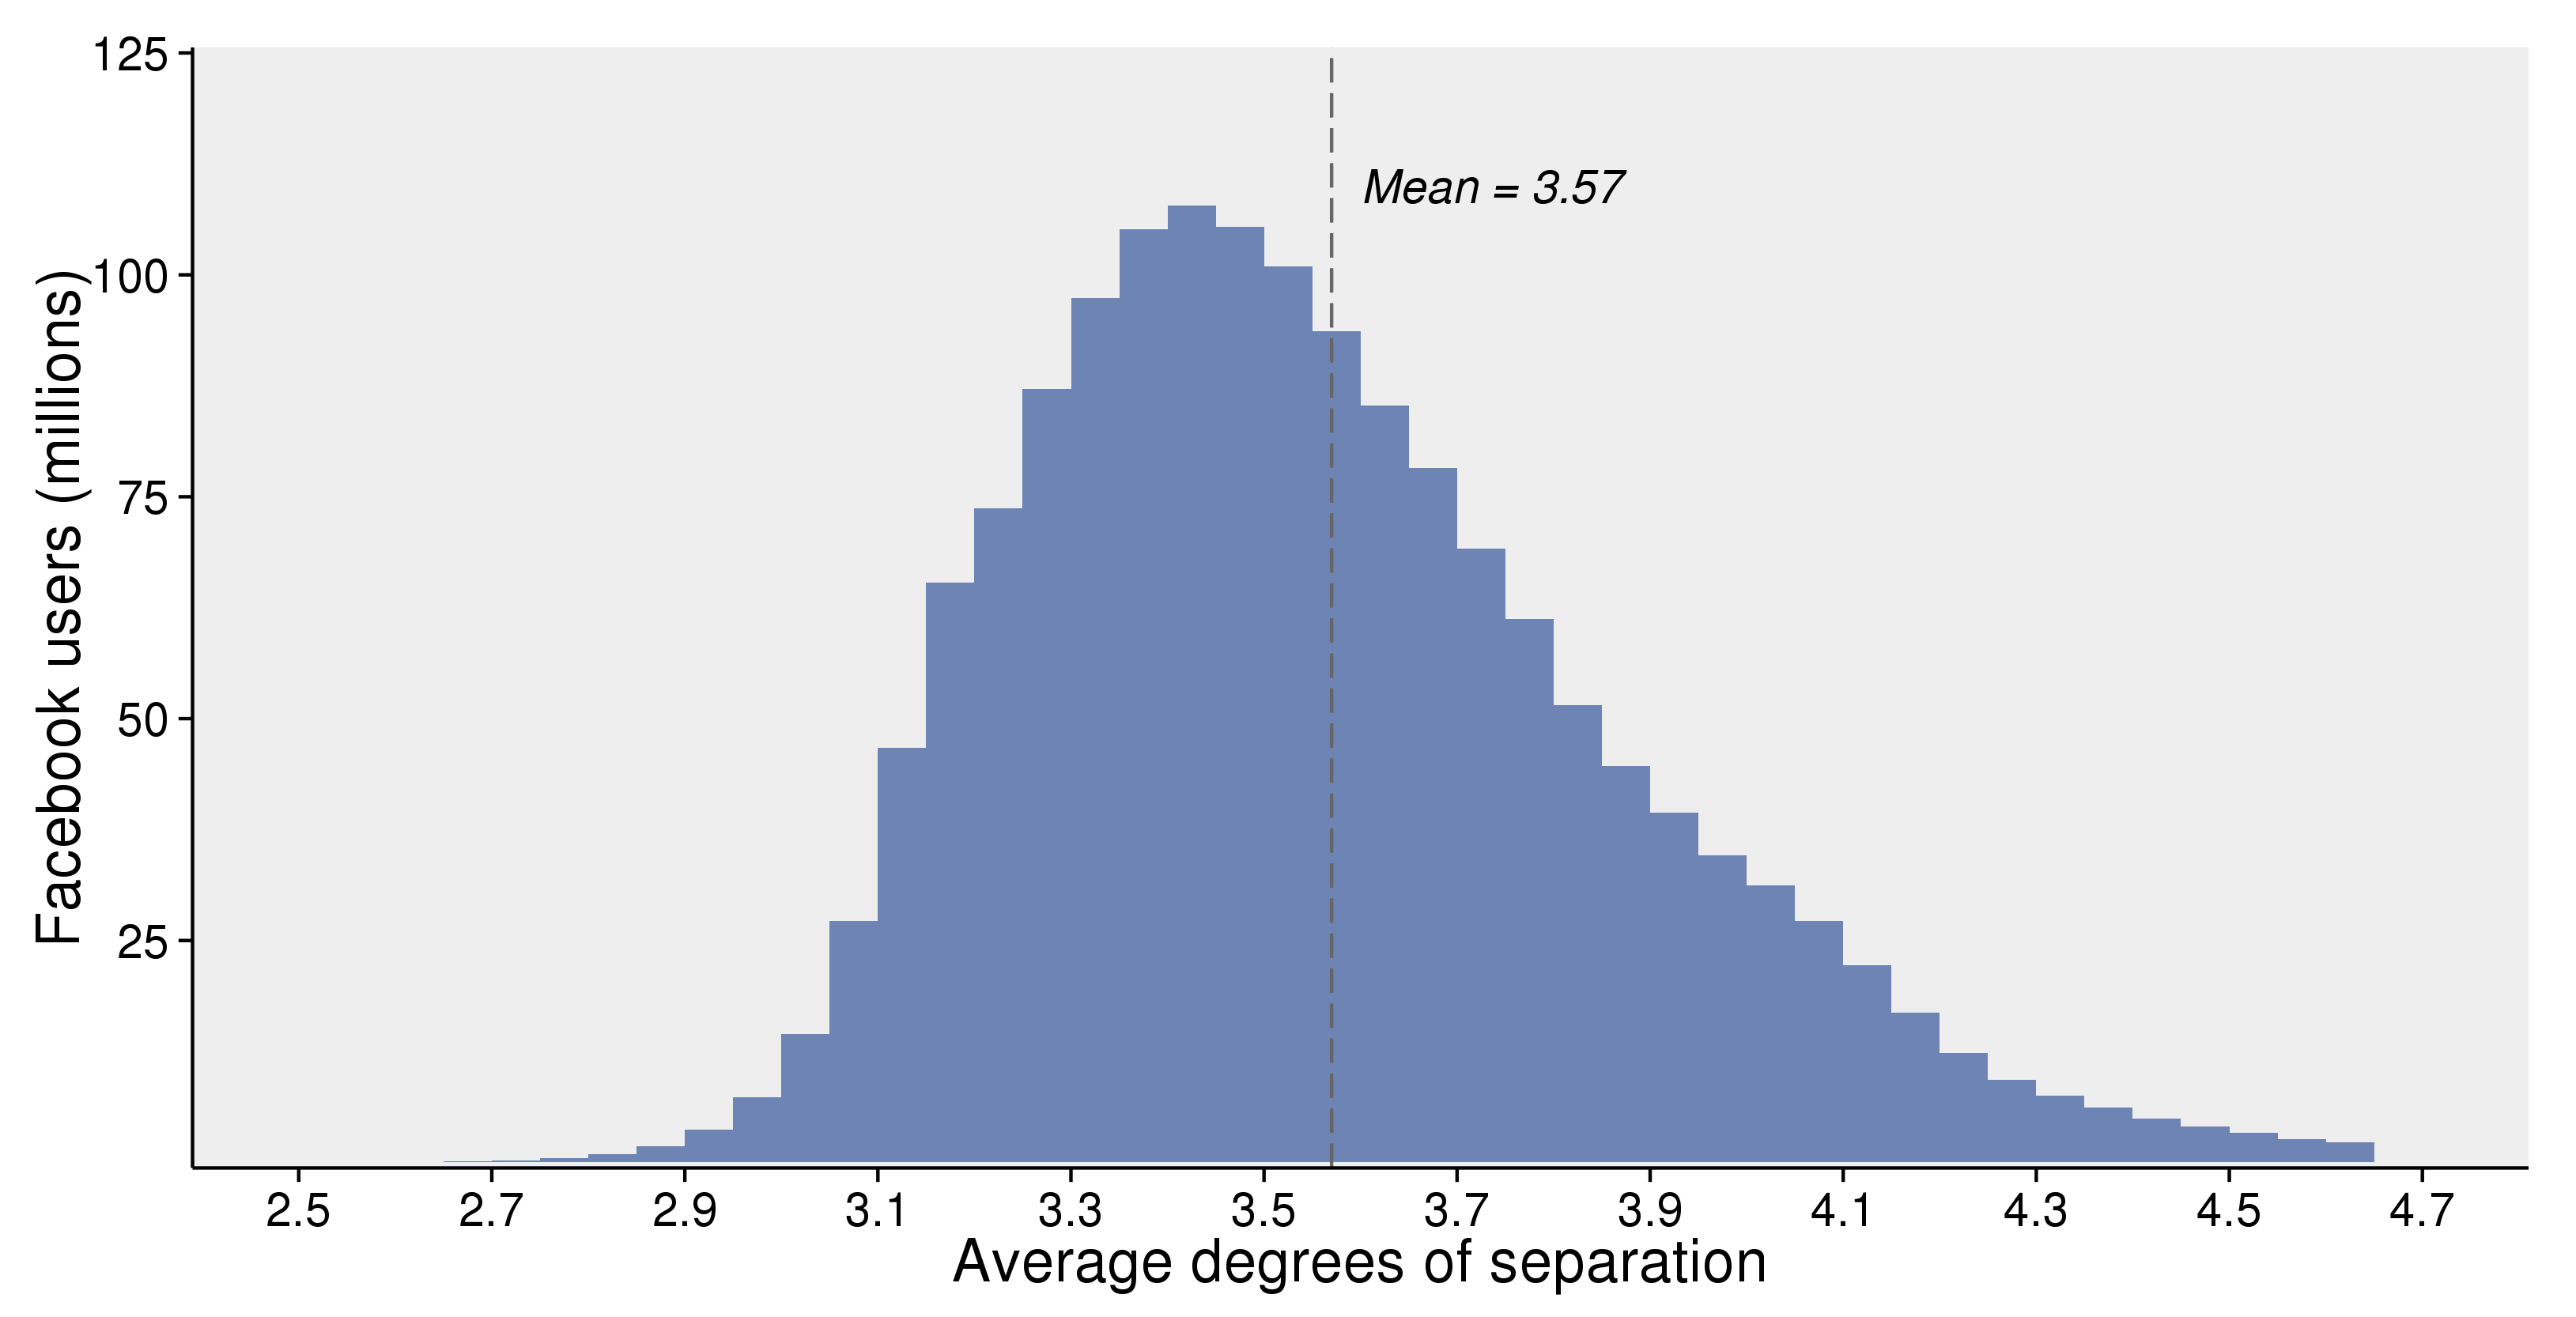
\includegraphics[width = \textwidth]{../img/facebook_separation}

{\footnotesize Fig 1. Estimated average degrees of separation between all people on FB.}
{\tiny (\url{https://research.facebook.com/blog/2016/2/three-and-a-half-degrees-of-separation/})}

\end{frame}
% ----------------------------------------------------

% ----------------------------------------------------
\begin{frame}
\frametitle{The original `theory'}
\centering

\textit{I read somewhere that everybody on this planet is separated by only six other people. Six degrees of separation. Between us and everybody else on this planet. The president of the United States. A gondolier in Venice. fill in the names.}\\\vspace{10pt}{\small Six Degrees of Separation, John Guare}

\vspace{20pt}

\begin{itemize}
  \item Do we have an answer?
\end{itemize}

\end{frame}
% ----------------------------------------------------

% ----------------------------------------------------
\begin{frame}
\frametitle{Bivariate relationships}
\centering

\begin{itemize}
  \item Examples?
\end{itemize}

\end{frame}
% ----------------------------------------------------

% ----------------------------------------------------
\begin{frame}
\frametitle{Bivariate relationship}
\centering

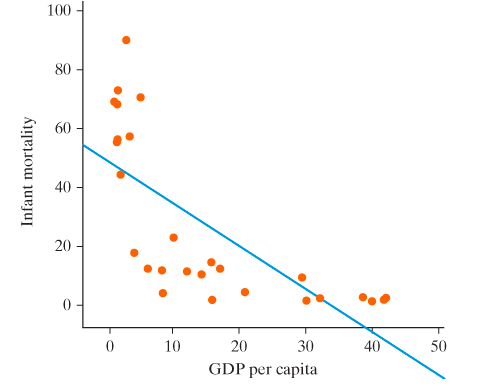
\includegraphics[width = 0.8\textwidth]{../img/scatter_GDP_mort}

\end{frame}
% ----------------------------------------------------

% ----------------------------------------------------
\begin{frame}
\frametitle{How many variables? Unit?}
\centering

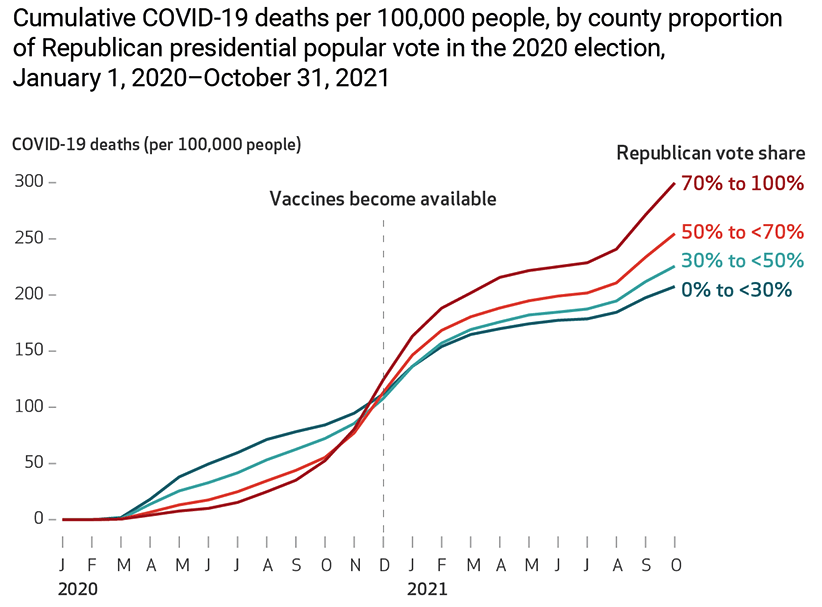
\includegraphics[width = \textwidth]{../img/covid_vote}

\end{frame}
% ----------------------------------------------------

% ----------------------------------------------------
\begin{frame}
\frametitle{How many variables? Unit?}
\centering

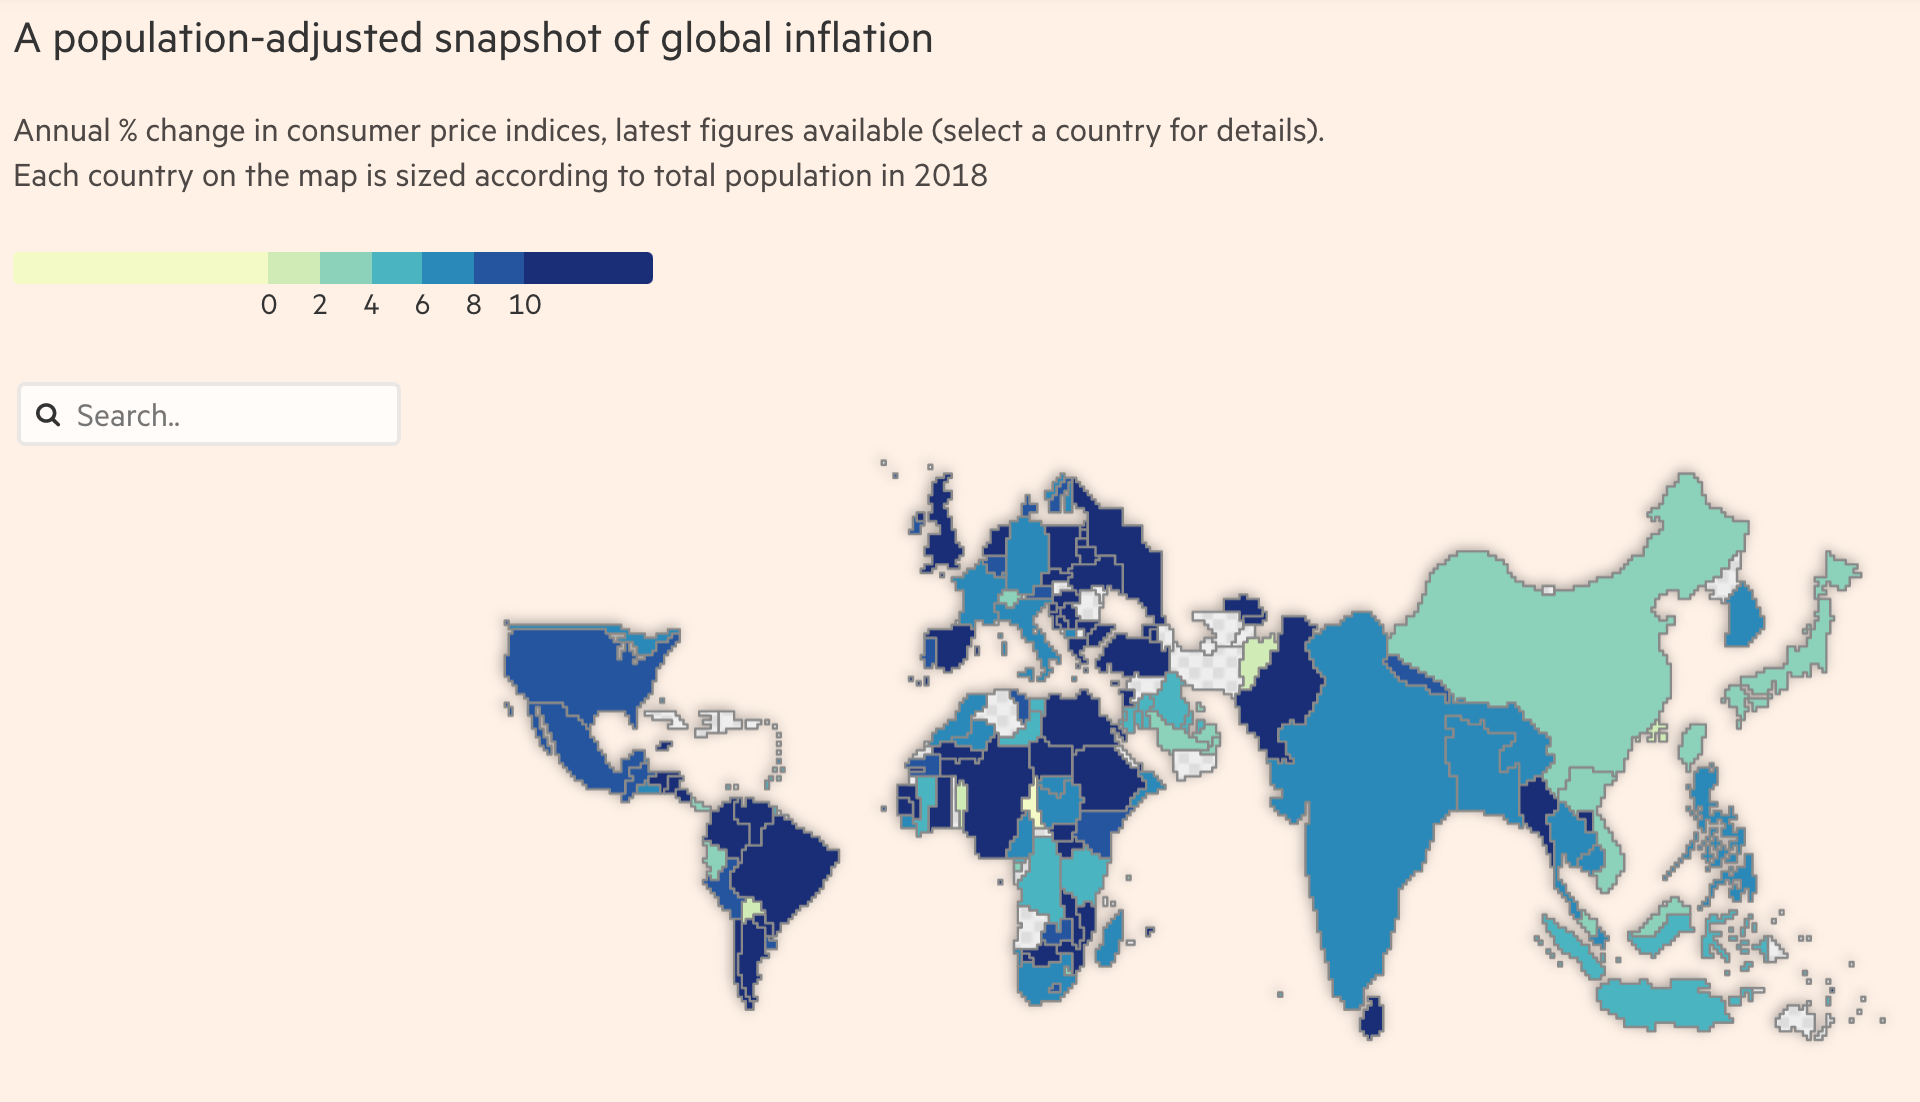
\includegraphics[width = \textwidth]{../img/global_inflation_ft}

\end{frame}
% ----------------------------------------------------

% ----------------------------------------------------
\begin{frame}
\frametitle{How many variables? Unit?}
\centering

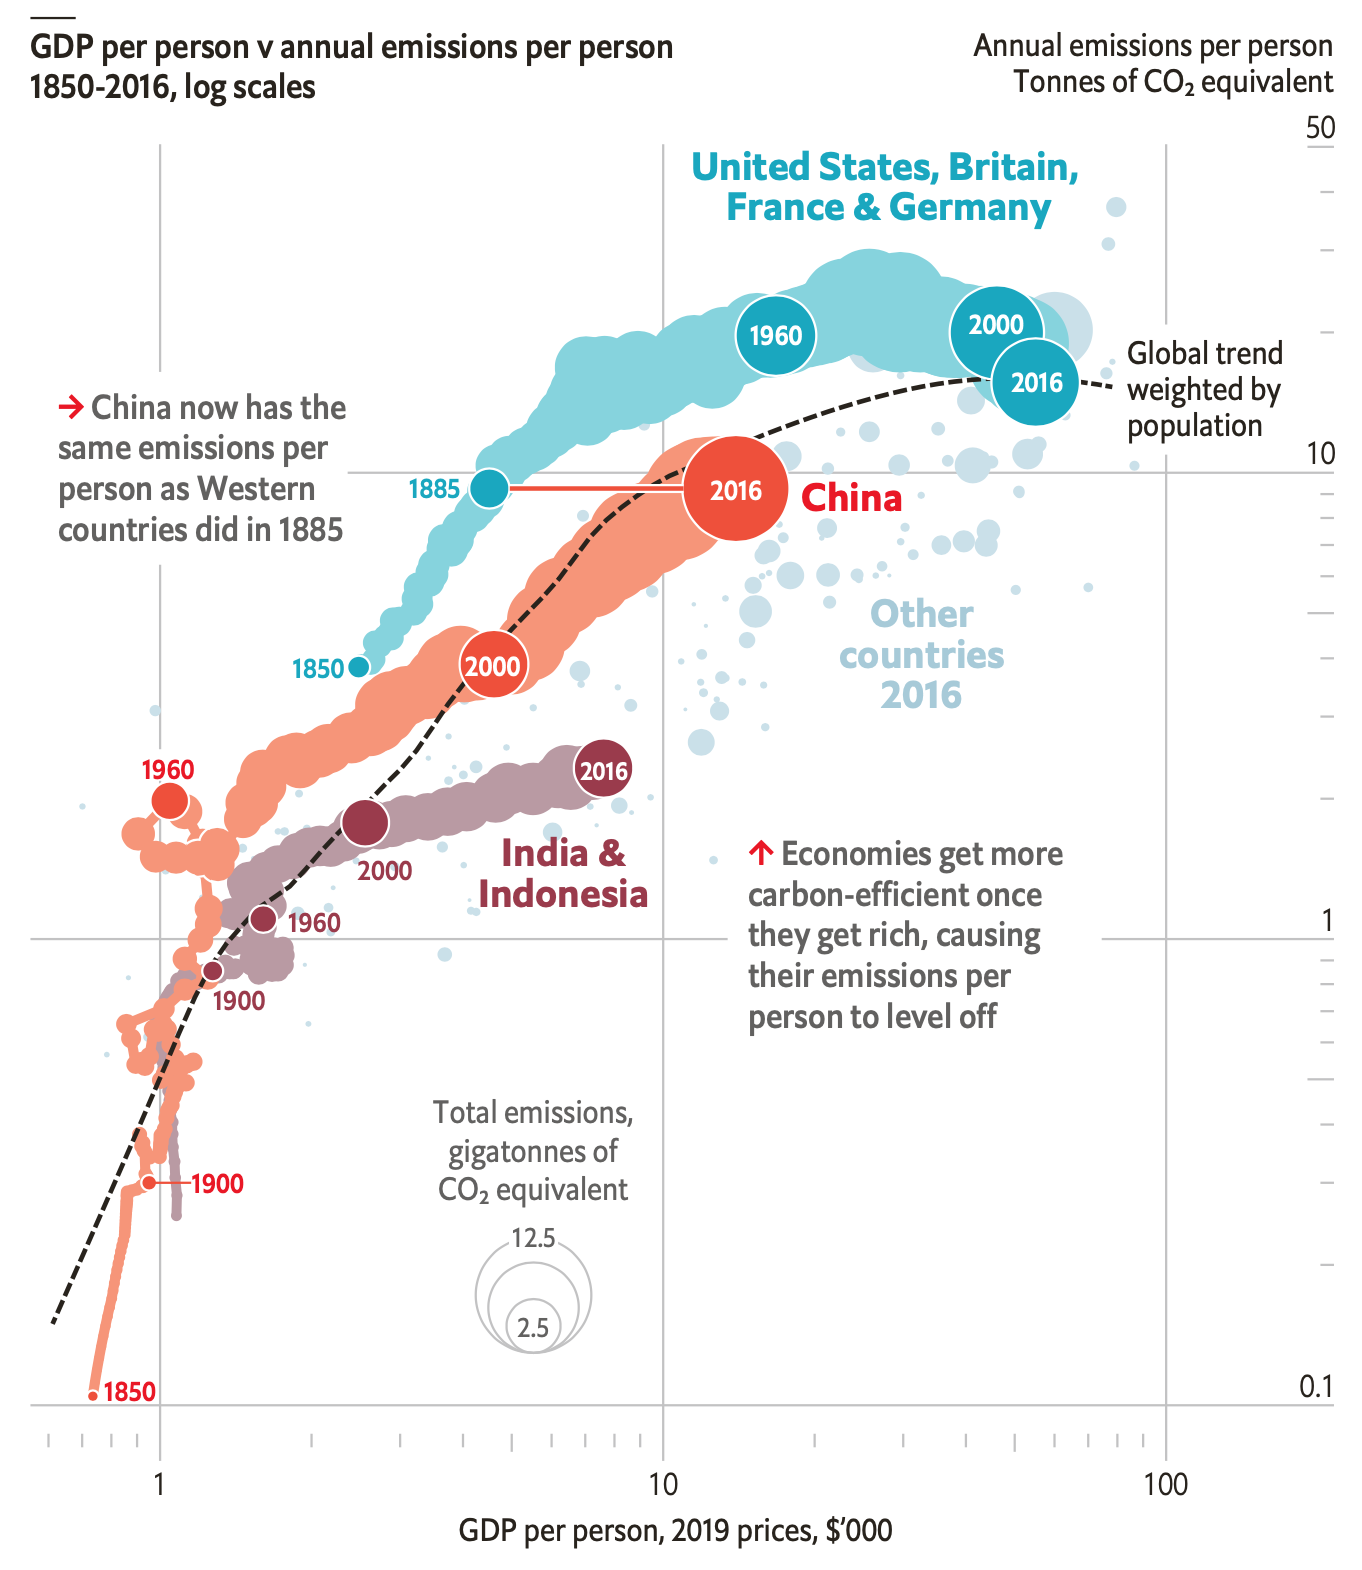
\includegraphics[width = 0.7\textwidth]{../img/emissions}

\end{frame}
% ----------------------------------------------------

% ----------------------------------------------------
\begin{frame}
\frametitle{Bivariate relationships}
\centering

\begin{itemize}[<+->]
  \item<1-> What do we use this for?
  \item<2-> Essentially, we are trying to detect whether two variables are dependent
  \begin{itemize}
    \item In other words, it's about conditional values: $E(Y|X)$
  \end{itemize}
  \item<3-> Example graph about infant mortality:
  \item<3->[] $E(IM|GDPpc = 1000)$?
  \item<3->[] $E(IM|GDPpc = 30000)$?
\end{itemize}

\end{frame}
% ----------------------------------------------------

% ----------------------------------------------------
\begin{frame}
\frametitle{Bivariate relationships}
\centering

\begin{itemize}[<+->]
  \item This is what statistics is about, and only this
  \item Even if it can get complicated: non-linear relationships, multivariate dependencies, etc
\end{itemize}

\end{frame}
% ----------------------------------------------------

% ----------------------------------------------------
\begin{frame}
\frametitle{Bivariate relationships}
\centering

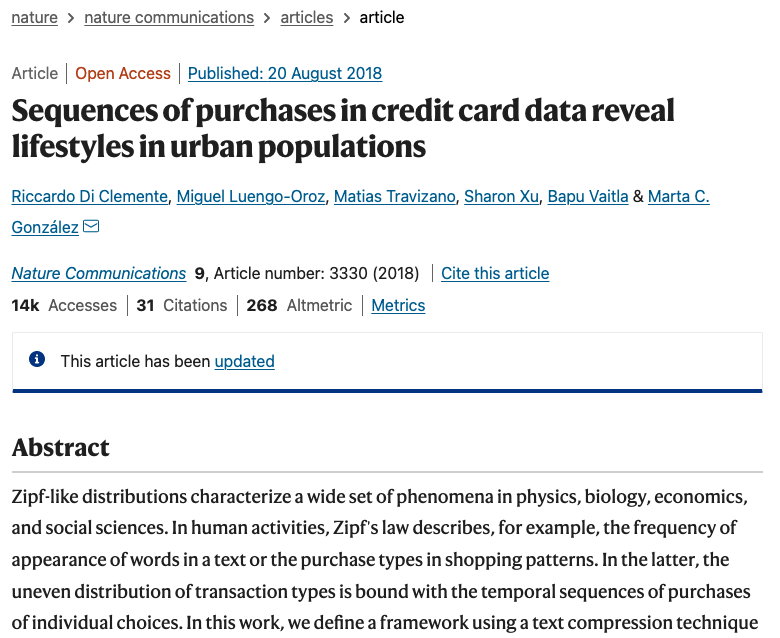
\includegraphics[width = 0.9\textwidth]{../img/nature_creditcard}

\end{frame}
% ----------------------------------------------------

% ----------------------------------------------------
\begin{frame}
\frametitle{Bivariate relationships}
\centering

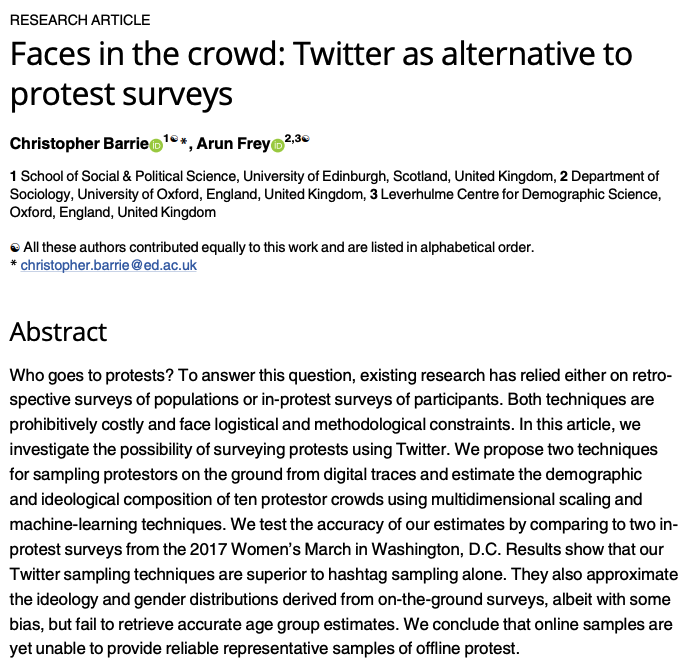
\includegraphics[width = 0.8\textwidth]{../img/twitter_protests}

\end{frame}
% ----------------------------------------------------

% ----------------------------------------------------
\begin{frame}
\frametitle{Describing relationships}
\centering

\begin{itemize}
  \item When we find a conditional relationship, we often say that $X$ \textit{explains} $Y$
  \item But these statistical relationships do \textit{not} tell us anything about cause and effect, only about conditional means (or $E(Y|X)$, or conditional conditional means if we also control for $Z$)
  \item We need another strategy to understand \textit{why}
\end{itemize}

\end{frame}
% ----------------------------------------------------

\section{Example: Wartime civilian deaths}

% ----------------------------------------------------
\begin{frame}
\frametitle{Practical example}
\centering

\begin{itemize}
  \item You want to test an argument about \textbf{wartime civilian deaths:}
  \begin{itemize}
    \item The intuition you have is that civilians will be more likely to be treated well (and not killed) by rebel groups during civil wars when they need their resources (e.g. labor) to survive
  \end{itemize}
  \item[]
  \item Clean up the theory, decide on the main concepts
  \item Develop different RQ at different levels
  \item How can we measure the main concepts? Variables?
  \item What answers could we get from the data?
    \begin{itemize}
      \item Are we learning something about our theory?
    \end{itemize}
\end{itemize}

\end{frame}
% ----------------------------------------------------

\section{Paper discussion}

% ----------------------------------------------------
\imageframe{../img/mullercrepon}
% ----------------------------------------------------

% ====================================================
\end{document}
